\documentclass[10pt, oneside]{book}
\ifdefined\HCode\else
\usepackage[Bjornstrup]{fncychap}
\fi
\usepackage[utf8]{inputenc}
\usepackage[T1]{fontenc}
\usepackage{graphicx}
\usepackage{fancyhdr}
\usepackage{xparse}
\usepackage{ifthen}
\usepackage{pdfpages}

% tikz settings
\usepackage{tikz}
\usetikzlibrary{shapes.geometric, arrows, shadows, decorations.text}
\tikzstyle{startstop} = [rectangle, rounded corners, minimum width=3cm, minimum height=1cm,text centered, draw=black, fill=red!30, drop shadow]
\tikzstyle{io} = [trapezium, trapezium left angle=70, trapezium right angle=110, minimum width=3cm, minimum height=1cm, text centered, draw=black, fill=blue!30]
\tikzstyle{process} = [rectangle, minimum width=3cm, minimum height=1cm, text centered, text width=3cm, draw=black, fill=orange!30]
\tikzstyle{decision} = [diamond, minimum width=1cm, minimum height=1cm, text centered, draw=black, fill=green!30]
\tikzstyle{arrow} = [thick,->,>=stealth]
\tikzstyle{line} = [draw, -latex']

% packages for code
\usepackage{verbatim}
\usepackage{minted}

% citation
\usepackage{cite}
\usepackage[colorlinks,citecolor=green]{hyperref}
\usepackage{cleveref}

\usepackage{xcolor}
\hypersetup{
  colorlinks,
  linkcolor = {red!50!black},
  citecolor = {blue!50!black},
  urlcolor = {blue!80!black}
}

\makeatletter
\@removefromreset{section}{chapter}
\makeatother
\renewcommand{\thesection}{\arabic{section}}

\input{lib/codeblock}
\input{lib/kernelsrc}

\author{Peter Jay Salzman, Michael Burian, Ori Pomerantz, Bob Mottram, Jim Huang}
\date{\today}
\title{The Linux Kernel Module Programming Guide}
\begin{document}

\maketitle
\ifdefined\HCode

\includegraphics{assets/cover-with-names.png}
\tableofcontents
\else
\pagestyle{empty}
\begin{tikzpicture}[remember picture, overlay]
  \node at (current page.center) {
\includegraphics[width=\paperwidth, height=\paperheight]{assets/cover.png}}; \\
  \node at (11, -9.5) {\Large \textbf{Peter Jay Salzman, Michael Burian,}}; \\
  \node at (11, -10.5) {\Large \textbf{Ori Pomerantz, Bob Mottram,}}; \\
  \node at (11, -11.5) {\Large \textbf{Jim Huang}};
\end{tikzpicture}
\tableofcontents
\fi

\chapter{Getting Started}
This chapter introduces the guide, outlines the basic development environment,
and builds up from the first loadable module. The emphasis is on getting a
working workflow in place before moving on to the broader kernel interfaces
used by more capable modules.

\section{Introduction}
\label{sec:introduction}
The Linux Kernel Module Programming Guide is a free book; you may reproduce or modify it under the terms of the \href{https://opensource.org/licenses/OSL-3.0}{Open Software License}, version 3.0.

This book is distributed in the hope that it would be useful, but without any warranty,
without even the implied warranty of merchantability or fitness for a particular purpose.

The author encourages wide distribution of this book for personal or commercial use,
provided the above copyright notice remains intact and the method adheres to the provisions of the \href{https://opensource.org/licenses/OSL-3.0}{Open Software License}.
In summary, you may copy and distribute this book free of charge or for a profit.
No explicit permission is required from the author for reproduction of this book in any medium, physical or electronic.

Derivative works and translations of this document must be placed under the Open Software License, and the original copyright notice must remain intact.
If you have contributed new material to this book, you must make the material and source code available for your revisions.
Please make revisions and updates available directly to the document maintainer, Ching-Chun (Jim) Huang <jserv@ccns.ncku.edu.tw>.
This will allow for the merging of updates and provide consistent revisions to the Linux community.

If you publish or distribute this book commercially, donations, royalties,
or printed copies are greatly appreciated by the author and the \href{https://tldp.org/}{Linux Documentation Project} (LDP).
Contributing in this way shows your support for free software and the LDP.
If you have questions or comments, please contact the address above.

\subsection{Authorship}
\label{sec:authorship}

The Linux Kernel Module Programming Guide was initially authored by Ori Pomerantz for Linux v2.2.
As the Linux kernel evolved, Ori's availability to maintain the document diminished.
Consequently, Peter Jay Salzman assumed the role of maintainer and updated the guide for Linux v2.4.
Similar constraints arose for Peter when tracking developments in Linux v2.6,
leading to Michael Burian joining as a co-maintainer to bring the guide up to speed with Linux v2.6.
Bob Mottram contributed to the guide by updating examples for Linux v3.8 and later.
Jim Huang then undertook the task of updating the guide for recent Linux versions (v5.0 and beyond),
along with revising the LaTeX document.
The guide now uses Linux v5.10 as its minimum supported baseline and aims to keep examples and guidance compatible across current long-term support kernels.

\subsection{Acknowledgements}
\label{sec:acknowledgements}

The following people have contributed corrections or good suggestions:

\begin{flushleft}
\input{contrib}
\end{flushleft}

\subsection{What Is A Kernel Module?}
\label{sec:kernelmod}

Involvement in the development of Linux kernel modules requires a foundation in the C programming language and a track record of creating conventional programs intended for process execution.
This pursuit delves into a domain where an unregulated pointer, if disregarded,
may potentially trigger the total elimination of an entire filesystem,
resulting in a scenario that necessitates a complete system reboot.

A Linux kernel module is precisely defined as a code segment capable of dynamic loading and unloading within the kernel as needed.
These modules enhance kernel capabilities without necessitating a system reboot.
A notable example is seen in the device driver module, which facilitates kernel interaction with hardware components linked to the system.
In the absence of modules, the prevailing approach leans toward monolithic kernels,
requiring direct integration of new functionalities into the kernel image.
This approach leads to larger kernels and necessitates kernel rebuilding and subsequent system rebooting when new functionalities are desired.

\subsection{Kernel module package}
\label{sec:packages}

Linux distributions provide the commands \sh|modprobe|, \sh|insmod| and \sh|depmod| within a package.

On Ubuntu/Debian GNU/Linux:
\begin{codebash}
sudo apt-get install build-essential kmod
\end{codebash}

On Arch Linux:
\begin{codebash}
sudo pacman -S gcc kmod
\end{codebash}

\subsection{What Modules are in my Kernel?}
\label{sec:modutils}

To discover what modules are already loaded within your current kernel, use the command \sh|lsmod|.
\begin{codebash}
lsmod
\end{codebash}

Modules are stored within the file \verb|/proc/modules|, so you can also see them with:
\begin{codebash}
cat /proc/modules
\end{codebash}

This can be a long list, and you might prefer to search for something particular.
To search for the \verb|fat| module:
\begin{codebash}
lsmod | grep fat
\end{codebash}

\subsection{Is there a need to download and compile the kernel?}
\label{sec:buildkernel}
To effectively follow this guide, there is no obligatory requirement for performing such actions.
Nonetheless, a prudent approach involves executing the examples within an isolated environment,
thus mitigating any potential risk of disrupting the system.

This guide includes a \verb|devtools/| directory that automates kernel module testing
inside a QEMU virtual machine.
It downloads a kernel source tree and a minimal BusyBox root filesystem, builds both,
and boots the result in QEMU with the host \verb|examples/| directory shared into the
guest via the 9p virtfs protocol.
You edit source files on your host and \sh|insmod| the compiled modules in the guest---no
disk images to manage, no root filesystem to rebuild.
See \Cref{sec:devtools_setup} for the complete setup procedure.

\subsection{Before We Begin}
\label{sec:preparation}
Before delving into code, certain matters require attention.
Variances exist among individuals' systems, and distinct personal approaches are evident.
The achievement of successful compilation and loading of the inaugural ``hello world'' program may,
at times, present challenges.
It is reassuring to note that overcoming the initial obstacle on the first attempt paves the way for subsequent endeavors to proceed seamlessly.

\begin{enumerate}
  \item Modversioning.
        A module compiled for one kernel will not load if a different kernel is booted,
        unless \cpp|CONFIG_MODVERSIONS| is enabled in the kernel.
        Module versioning will be discussed later in this guide.
        Until module versioning is covered, the examples in this guide may not work correctly if running a kernel with modversioning turned on.
        However, most stock Linux distribution kernels come with modversioning enabled.
        If difficulties arise when loading the modules due to versioning errors, consider compiling a kernel with modversioning turned off.

  \item Using the X Window System.
        It is highly recommended to extract, compile, and load all the examples discussed in this guide from a console.
        Working on these tasks within the X Window System is discouraged.

        Modules cannot directly print to the screen like \cpp|printf()| can,
        but they can log information and warnings to the kernel's log ring buffer.
        This output is \emph{not} automatically displayed on any console or terminal.
        To view kernel module messages, you must use \sh|dmesg| to read the kernel log ring buffer,
        or check the systemd journal with \sh|journalctl -k| for kernel messages.
        Refer to \Cref{sec:helloworld} for more information.
        The terminal or environment from which you load the module does not affect where the output goes—it always goes to the kernel log.
  \item SecureBoot.
        Numerous modern computers arrive pre-configured with UEFI SecureBoot enabled—an essential security standard ensuring booting exclusively through trusted software endorsed by the original equipment manufacturer.
        Certain Linux distributions even ship with the default Linux kernel configured to support SecureBoot.
        In these cases, the kernel module necessitates a signed security key.

        Failing that, an attempt to insert your first ``hello world'' module would result in the message: ``\emph{ERROR: could not insert module}''.
        If this message ``\emph{Lockdown: insmod: unsigned module loading is restricted;
        see man kernel lockdown.7}'' appears in the \sh|dmesg| output,
        the simplest approach involves disabling UEFI SecureBoot from the boot menu of your PC or laptop,
        allowing the successful insertion of the ``hello world'' module.
        Naturally, an alternative involves undergoing intricate procedures such as generating keys, system key installation,
        and module signing to achieve functionality.
        However, this intricate process is less appropriate for beginners. If interested,
        more detailed steps for \href{https://wiki.debian.org/SecureBoot}{SecureBoot} can be explored and followed.
        In the real world—especailly in enterprise environment, production servers, or laptops where your IT staffs mandate strict security—it is not eligible to disable SecureBoot.
        If you ever encounter such situations, visit \Cref{sec:secure_boot_signing_guide} for a SecureBoot signing thorough guide.
\end{enumerate}

If you are building your own kernel for module development, these \verb|.config| options are useful for debugging and development:
\begin{itemize}
  \item \cpp|CONFIG_DEBUG_INFO|: include debug symbols so \sh|gdb|, \sh|addr2line|, and \sh|objdump| can map crash addresses to source lines.
  \item \cpp|CONFIG_DYNAMIC_DEBUG|: enable runtime-switchable \cpp|pr_debug()| statements (see \Cref{sec:printk}).
  \item \cpp|CONFIG_KASAN| (Kernel Address Sanitizer): instruments memory accesses to detect out-of-bounds, use-after-free, and other memory errors at the cost of roughly 2$\times$ memory usage and some CPU overhead.
  \item \cpp|CONFIG_LOCKDEP| (lock dependency checker): detects potential deadlocks (lock order inversions, sleeping under spinlocks, wrong lock type for context) at runtime, before they actually hang the system.
  \item \cpp|CONFIG_DEBUG_ATOMIC_SLEEP|: flags attempts to sleep in atomic context, catching the most common spinlock misuse.
  \item \cpp|CONFIG_MODULE_FORCE_UNLOAD|: allows \sh|rmmod -f| as a last resort during development, but use it with care because force-unloading can hide lifetime bugs and leave the kernel in an inconsistent state.
\end{itemize}
The QEMU-based environment described below already enables
\cpp|CONFIG_DEBUG_INFO| and \cpp|CONFIG_MODULE_FORCE_UNLOAD|; enable the
others explicitly if you want those extra diagnostics.

\subsection{QEMU-Based Development Environment}
\label{sec:devtools_setup}
An alternative to installing kernel headers on your host and loading modules
into your running kernel is to use the QEMU-based development environment
provided under \verb|devtools/|.
This approach is especially useful on machines where you cannot (or prefer not to)
load arbitrary kernel modules (for example, hosts with SecureBoot enabled, corporate
laptops, or macOS workstations).

The setup compiles a minimal Linux kernel with module, debugfs, procfs, and 9p
filesystem support, along with a statically linked BusyBox initramfs.
QEMU boots this kernel and shares the project directory into the guest via the 9p
virtfs protocol, so every file you edit on the host is immediately visible inside the
virtual machine.

\textbf{Prerequisites.}
The kernel and BusyBox builds require a Linux host (or a Linux environment such as
Docker or \href{https://lima-vm.io/}{Lima} on macOS).
QEMU itself runs natively on Linux and macOS.

\begin{codebash}
# Debian/Ubuntu: install the build toolchain and QEMU
sudo apt-get install build-essential flex bison bc libelf-dev libssl-dev cpio qemu-system-x86

# macOS: install QEMU (kernel build runs inside Lima or Docker)
brew install qemu
\end{codebash}

\textbf{One-time setup} (downloads a kernel tarball and BusyBox, builds both, and
packs an initramfs):
\begin{codebash}
devtools/setup.sh
\end{codebash}

\textbf{Building modules} against the QEMU kernel (must be run on Linux):
\begin{codebash}
devtools/build-modules.sh
\end{codebash}

\textbf{Interactive testing.}
Boot QEMU and get a shell inside the guest.
The project tree is mounted at \verb|/mnt/lkmpg/|, with compiled modules at
\verb|/mnt/lkmpg/examples/*.ko|:
\begin{codebash}
devtools/boot.sh
# Inside the guest:
insmod /mnt/lkmpg/examples/hello-1.ko
dmesg | tail
rmmod hello_1
\end{codebash}

\textbf{Automated testing.}
Build all modules and run \sh|insmod|/\sh|rmmod| for every module in a single
command.
Modules listed in \verb|.ci/non-working| are automatically skipped:
\begin{codebash}
devtools/test-modules.sh
\end{codebash}

\textbf{Kernel debugging with GDB.}
GDB requires the \verb|vmlinux| image with debug symbols.
Prebuilt setups omit it for size; rebuild from source first:
\begin{codebash}
LKMPG_NO_PREBUILT=1 devtools/setup.sh
\end{codebash}

Then start QEMU paused and attach GDB from a second terminal:
\begin{codebash}
# Terminal 1: QEMU waits for a debugger connection
devtools/boot.sh --gdb

# Terminal 2: connect GDB
gdb devtools/.cache/kernel-build/vmlinux \
    -ex "target remote :1234" \
    -ex "break do_init_module" \
    -ex continue
\end{codebash}
When you \sh|insmod| a module in the guest, GDB will break at the module
initialization entry point.

\textbf{Overriding defaults.}
Create \verb|devtools/config.local| (gitignored) to change the kernel version,
QEMU memory size, or other settings:
\begin{code}
KERNEL_VERSION="6.6.70"
QEMU_MEM="1G"
\end{code}
Rerun \verb|devtools/setup.sh| after changing \verb|KERNEL_VERSION|.

\section{Kernel Headers}
\label{sec:headers}
Before building anything, it is necessary to install the header files for the kernel.
If you are using the QEMU-based environment described in \Cref{sec:devtools_setup},
the kernel headers are built automatically by \verb|devtools/setup.sh| and you can
skip this step.

On Ubuntu/Debian GNU/Linux:
\begin{codebash}
sudo apt-get update
apt-cache search linux-headers-`uname -r`
\end{codebash}

The following command provides information about the available kernel header files.
Then, for example:
\begin{codebash}
sudo apt-get install linux-headers-`uname -r`
\end{codebash}

On Arch Linux:
\begin{codebash}
sudo pacman -S linux-headers
\end{codebash}

On Fedora:
\begin{codebash}
sudo dnf install kernel-devel kernel-headers
\end{codebash}

\section{Examples}
\label{sec:examples}
All the examples from this document are available within the \verb|examples| subdirectory.

To build all examples at once, run \sh|make| from within the \verb|examples/| directory
(requires kernel headers installed, see \Cref{sec:headers}), or use the QEMU-based
environment:
\begin{codebash}
devtools/build-modules.sh
\end{codebash}

To run automated \sh|insmod|/\sh|rmmod| tests for every module inside QEMU:
\begin{codebash}
devtools/test-modules.sh
\end{codebash}

Should compile errors occur, it may be due to a more recent kernel version being in use,
or there might be a need to install the corresponding kernel header files.

\section{Hello World}
\label{sec:helloworld}
\subsection{The Simplest Module}
\label{sec:org2d3e245}
Most individuals beginning their programming journey typically start with some variant of a \emph{hello world} example.
It is unclear what the outcomes are for those who deviate from this tradition, but it seems prudent to adhere to it.
The learning process will begin with a series of hello world programs that illustrate various fundamental aspects of writing a kernel module.

Presented next is the simplest possible module.

Make a test directory:
\begin{codebash}
mkdir -p ~/develop/kernel/hello-1
cd ~/develop/kernel/hello-1
\end{codebash}

Paste this into your favorite editor and save it as \verb|hello-1.c|:

\samplec{examples/hello-1.c}

Now you will need a \verb|Makefile|. If you copy and paste this, change the indentation to use \textit{tabs}, not spaces.

\begin{code}
obj-m += hello-1.o

PWD := $(CURDIR)

all:
	$(MAKE) -C /lib/modules/$(shell uname -r)/build M=$(PWD) modules

clean:
	$(MAKE) -C /lib/modules/$(shell uname -r)/build M=$(PWD) clean
\end{code}

In \verb|Makefile|, \verb|$(CURDIR)| can be set to the absolute pathname of the current working directory (after all \verb|-C| options are processed, if any).
See more about \verb|CURDIR| in \href{https://www.gnu.org/software/make/manual/make.html}{GNU make manual}.

And finally, just run \verb|make| directly.

\begin{codebash}
make
\end{codebash}

If there is no \verb|PWD := $(CURDIR)| statement in the Makefile, then it may not compile correctly with \verb|sudo make|.
This is because some environment variables are specified by the security policy and cannot be inherited.
The default security policy is \verb|sudoers|.
In the \verb|sudoers| security policy, \verb|env_reset| is enabled by default, which restricts environment variables.
Specifically, path variables are not retained from the user environment;
they are set to default values (for more information, see: \href{https://www.sudo.ws/docs/man/sudoers.man/}{sudoers manual}).
You can see the environment variable settings by:

\begin{verbatim}
$ sudo -s
# sudo -V
\end{verbatim}

Here is a simple Makefile as an example to demonstrate the problem mentioned above.

\begin{code}
all:
	echo $(PWD)
\end{code}

Then, we can use the \verb|-p| flag to print out the environment variable values from the Makefile.

\begin{verbatim}
$ make -p | grep PWD
PWD = /home/ubuntu/temp
OLDPWD = /home/ubuntu
	echo $(PWD)
\end{verbatim}

The \verb|PWD| variable will not be inherited with \verb|sudo|.

\begin{verbatim}
$ sudo make -p | grep PWD
	echo $(PWD)
\end{verbatim}

However, there are three ways to solve this problem.

\begin{enumerate}
  \item {
  You can use the \verb|-E| flag to temporarily preserve them.

  \begin{codebash}
    $ sudo -E make -p | grep PWD
    PWD = /home/ubuntu/temp
    OLDPWD = /home/ubuntu
    echo $(PWD)
  \end{codebash}
  }

  \item {
  You can disable \verb|env_reset| by editing \verb|/etc/sudoers| as root using \verb|visudo|.

  \begin{code}
  ## sudoers file.
  ##
  ...
  Defaults env_reset
  ## Change env_reset to !env_reset in previous line to keep all environment variables
  \end{code}

  Then execute \verb|env| and \verb|sudo env| individually.

  \begin{codebash}
    # disable the env_reset
    echo "user:" > non-env_reset.log; env >> non-env_reset.log
    echo "root:" >> non-env_reset.log; sudo env >> non-env_reset.log
    # enable the env_reset
    echo "user:" > env_reset.log; env >> env_reset.log
    echo "root:" >> env_reset.log; sudo env >> env_reset.log
  \end{codebash}

  You can view and compare these logs to find differences between \verb|env_reset| and \verb|!env_reset|.
  }

  \item {You can preserve environment variables by appending them to \verb|env_keep| in \verb|/etc/sudoers|.

  \begin{code}
  Defaults env_keep += "PWD"
  \end{code}

  After applying the above change, you can check the environment variable settings by:

  \begin{verbatim}
    $ sudo -s
    # sudo -V
  \end{verbatim}
  }
\end{enumerate}

If all goes smoothly you should then find that you have a compiled \verb|hello-1.ko| module.
You can find info on it with the command:
\begin{codebash}
modinfo hello-1.ko
\end{codebash}

At this point the command:
\begin{codebash}
lsmod | grep hello
\end{codebash}

should return nothing.
You can try loading your new module with:
\begin{codebash}
sudo insmod hello-1.ko
\end{codebash}

The dash character will get converted to an underscore, so when you again try:
\begin{codebash}
lsmod | grep hello
\end{codebash}

You should now see your loaded module. It can be removed again with:
\begin{codebash}
sudo rmmod hello_1
\end{codebash}

Notice that the dash was replaced by an underscore.
To see the module's output messages, use \sh|dmesg| to view the kernel log ring buffer:
\begin{codebash}
sudo dmesg | tail -10
\end{codebash}

You should see messages like ``Hello world 1.'' and ``Goodbye world 1.'' from your module.
Alternatively, you can check the systemd journal for kernel messages:
\begin{codebash}
journalctl --since "1 hour ago" | grep kernel
\end{codebash}

If you are using the QEMU environment from \Cref{sec:devtools_setup} instead, the
same exercise looks like this:
\begin{codebash}
devtools/build-modules.sh        # compile all examples
devtools/boot.sh                 # boot into the QEMU guest
# inside the guest:
insmod /mnt/lkmpg/examples/hello-1.ko
dmesg | tail
rmmod hello_1
\end{codebash}
No \sh|sudo| is needed because the guest runs as root.

You now know the basics of creating, compiling, installing and removing modules.
Now for more of a description of how this module works.

Kernel modules must have at least two functions: a "start" (initialization) function called \cpp|init_module()| which is called when the module is \sh|insmod|ed into the kernel,
and an "end" (cleanup) function called \cpp|cleanup_module()| which is called just before it is removed from the kernel.
Actually, things have changed starting with kernel 2.3.13.
% TODO: adjust the section anchor
You can now use whatever name you like for the start and end functions of a module,
and you will learn how to do this in \Cref{sec:hello_n_goodbye}.
In fact, the new method is the preferred method.
The old \cpp|init_module()| and \cpp|cleanup_module()| have been deprecated for x86 systems with indirect branch tracking (IBT) enabled starting from \href{https://github.com/torvalds/linux/commit/4fab2d76}{commit 4fab2d76} in kernel 6.15, causing build failures.
However, many existing examples still use these names for their start and end functions.

Typically, \cpp|init_module()| either registers a handler for something with the kernel, 
or it replaces one of the kernel functions with its own code (usually code to do something and then call the original function).
The \cpp|cleanup_module()| function is supposed to undo whatever \cpp|init_module()| did, so the module can be unloaded safely.

Lastly, every kernel module needs to include \src{include/linux/module.h}.
% TODO: adjust the section anchor
We needed to include \src{include/linux/printk.h} only for the macro expansion for the \cpp|pr_alert()| log level, which you'll learn about in \Cref{sec:printk}.

\begin{enumerate}
  \item A point about coding style.
        Another thing that may not be immediately obvious to anyone getting started with kernel programming is that indentation within your code should use \textbf{tabs} and \textbf{not spaces}.
        It is one of the coding conventions of the kernel.
        You may not like it, but you will need to get used to it if you ever submit a patch upstream.

  \item Introducing print macros.
  \label{sec:printk}
        In the beginning there was \cpp|printk|, usually followed by a priority such as \cpp|KERN_INFO| or \cpp|KERN_DEBUG|.
        More recently, this can also be expressed in abbreviated form using a set of print macros, such as \cpp|pr_info| and \cpp|pr_debug|.
        This just saves some mindless keyboard bashing and looks a bit neater.
        They can be found within \src{include/linux/printk.h}.
        Take time to read through the available priority macros.

        \textbf{Important:} These functions write to the kernel log ring buffer, \emph{not} directly to any terminal or console.
        To view the output from your kernel modules, you must use \sh|dmesg| or \sh|journalctl -k|.

        The kernel log buffer is a fixed-size circular buffer (sized via \cpp|CONFIG_LOG_BUF_SHIFT| in the kernel configuration).
        Excessive logging can overflow the buffer and push out earlier messages before they are read.
        In hot paths (interrupt handlers, per-packet processing, or tight loops), use the rate-limited variants \cpp|pr_info_ratelimited()|, \cpp|pr_warn_ratelimited()|, etc., or the explicit \cpp|printk_ratelimit()| guard, to avoid flooding the log and slowing down the system due to console output overhead.
        See \src{include/linux/ratelimit.h} for details.

        For development, \cpp|pr_debug()| is particularly useful.
        When the kernel is compiled with \cpp|CONFIG_DYNAMIC_DEBUG|, \cpp|pr_debug()| calls are compiled in but disabled by default.
        You can selectively enable them at runtime without recompiling or reloading the module by writing to \verb|/sys/kernel/debug/dynamic_debug/control|:
        \begin{codebash}
echo "module mymodule +p" > /sys/kernel/debug/dynamic_debug/control
        \end{codebash}
        The \verb|+p| flag activates printing; \verb|-p| disables it.
        You can filter by file, function, or line number.
        See \src{Documentation/admin-guide/dynamic-debug-howto.rst} for the full syntax.

  \item About Compiling.
        Kernel modules need to be compiled a bit differently from regular userspace apps.
        Former kernel versions required us to care much about these settings, which are usually stored in Makefiles.
        Although hierarchically organized, many redundant settings accumulated in sublevel Makefiles and made them large and rather difficult to maintain.
        Fortunately, there is a new way of doing these things, called kbuild, and the build process for external loadable modules is now fully integrated into the standard kernel build mechanism.
        To learn more about how to compile modules which are not part of the official kernel (such as all the examples you will find in this guide), see file \src{Documentation/kbuild/modules.rst}.

        Additional details about Makefiles for kernel modules are available in \src{Documentation/kbuild/makefiles.rst}.
        Be sure to read this and the related files before starting to hack Makefiles. It will probably save you lots of work.

\begin{quote}
Here is another exercise for the reader.
See that comment above the return statement in \cpp|init_module()|?
Change the return value to something negative, recompile and load the module again.
What happens?
\end{quote}
\end{enumerate}

\subsection{Hello and Goodbye}
\label{sec:hello_n_goodbye}
In early kernel versions you had to use the \cpp|init_module| and \cpp|cleanup_module| functions, as in the first hello world example,
but these days you can name those anything you want by using the \cpp|module_init| and \cpp|module_exit| macros.
These macros are defined in \src{include/linux/module.h}.
The only requirement is that your init and cleanup functions must be defined before calling those macros, otherwise you will get compilation errors.
Here is an example of this technique:

\samplec{examples/hello-2.c}

So now we have two real kernel modules under our belt. Adding another module is as simple as this:

\begin{code}
obj-m += hello-1.o
obj-m += hello-2.o

PWD := $(CURDIR)

all:
	$(MAKE) -C /lib/modules/$(shell uname -r)/build M=$(PWD) modules

clean:
	$(MAKE) -C /lib/modules/$(shell uname -r)/build M=$(PWD) clean
\end{code}

Now have a look at \src{drivers/char/Makefile} for a real world example.
As you can see, some things got hardwired into the kernel (\verb|obj-y|) but where have all those \verb|obj-m| gone?
Those familiar with shell scripts will easily be able to spot them.
For those who are not, the \verb|obj-$(CONFIG_FOO)| entries you see everywhere expand into \verb|obj-y| or \verb|obj-m|,
depending on whether the \verb|CONFIG_FOO| variable has been set to \verb|y| or \verb|m|.
While we are at it, those were exactly the kind of variables that you have set in the \verb|.config| file in the top-level directory of the Linux kernel source tree,
the last time you ran \sh|make menuconfig| or something similar.

\subsection{The \_\_init and \_\_exit Macros}
\label{sec:init_n_exit}
The \cpp|__init| macro causes the init function to be discarded and its memory freed once the init function finishes for built-in drivers.
For loadable modules, \cpp|__init| still places the function into an init-only section, \cpp|do_free_init| may still be observable during module loading even without \cpp|__init|.
If you think about when the init function is invoked, this makes perfect sense.

There is also an \cpp|__initdata| which works similarly to \cpp|__init| but for init variables rather than functions.

The \cpp|__exit| macro causes the omission of the function when the module is built into the kernel, and like \cpp|__init|, has no effect for loadable modules.
Again, if you consider when the cleanup function runs, this makes complete sense; built-in drivers do not need a cleanup function, while loadable modules do.

These macros are defined in \src{include/linux/init.h} and serve to free up kernel memory.
When you boot your kernel and see something like Freeing unused kernel memory: 236k freed, this is precisely what the kernel is freeing.

\samplec{examples/hello-3.c}

\subsection{Licensing and Module Documentation}
\label{sec:modlicense}
Honestly, who loads or even cares about proprietary modules?
If you do then you might have seen something like this:
\begin{verbatim}
$ sudo insmod xxxxxx.ko
loading out-of-tree module taints kernel.
module license 'unspecified' taints kernel.
\end{verbatim}

You can use a few macros to indicate the license for your module.
Some examples are "GPL", "GPL v2", "GPL and additional rights", "Dual BSD/GPL", "Dual MIT/GPL", "Dual MPL/GPL" and "Proprietary".
They are defined within \src{include/linux/module.h}.

To reference what license you are using, a macro is available called \cpp|MODULE_LICENSE|.
This and a few other macros describing the module are illustrated in the example below.

\samplec{examples/hello-4.c}

\subsection{Passing Command Line Arguments to a Module}
\label{sec:modparam}
Modules can take command line arguments, but not with the argc/argv you might be used to.

To allow arguments to be passed to your module, declare the variables that will take the values of the command line arguments as global and then use the \cpp|module_param()| macro (defined in \src{include/linux/moduleparam.h}) to set the mechanism up.
At runtime, \sh|insmod| will fill the variables with any command line arguments that are given, like \sh|insmod mymodule.ko myvariable=5|.
The variable declarations and macros should be placed at the beginning of the module for clarity.
The example code should clear up my admittedly lousy explanation.

The \cpp|module_param()| macro takes 3 arguments: the name of the variable, its type and permissions for the corresponding file in sysfs.
Integer types can be signed as usual or unsigned. If you would like to use arrays of integers or strings,
see \cpp|module_param_array()| and \cpp|module_param_string()|.

\begin{code}
int myint = 3;
module_param(myint, int, 0);
\end{code}

Arrays are supported too, but things are a bit different now than they were in the olden days.
To keep track of the number of parameters, you need to pass a pointer to a count variable as the third parameter.
At your option, you could also ignore the count and pass \cpp|NULL| instead.
We show both possibilities here:

\begin{code}
int myintarray[2];
module_param_array(myintarray, int, NULL, 0); /* not interested in count */

short myshortarray[4];
int count;
module_param_array(myshortarray, short, &count, 0); /* put count into "count" variable */
\end{code}

A good use for this is to have the module variable's default values set, like a port or IO address.
If the variables contain the default values, then perform autodetection (explained elsewhere).
Otherwise, keep the current value.
This will be made clear later on.

Lastly, there is a macro function, \cpp|MODULE_PARM_DESC()|, that is used to document arguments that the module can take.
It takes two parameters: a variable name and a free form string describing that variable.

\samplec{examples/hello-5.c}

If you need to validate a parameter or react whenever it changes, use \cpp|module_param_cb()|.
This variant takes four arguments: the parameter name, a pointer to a \cpp|struct kernel_param_ops|,
an argument pointer (typically the address of the backing variable), and the sysfs permissions.
The callbacks stored in \cpp|struct kernel_param_ops| let you override the \cpp|set| and \cpp|get|
operations instead of relying on the default helpers such as \cpp|param_set_int()| and \cpp|param_get_int()|.
With non-zero permissions, the parameter is also exposed through sysfs so the same callbacks can run after the module has already been loaded.

\begin{code}
static int watched = 42;

static int watched_set(const char *val, const struct kernel_param *kp)
{
    int ret = param_set_int(val, kp);

    if (ret)
        return ret;

    pr_info("watched updated to %d\n", watched);
    return 0;
}

static const struct kernel_param_ops watched_ops = {
    .set = watched_set,
    .get = param_get_int,
};

module_param_cb(watched, &watched_ops, &watched, 0644);
\end{code}

The full example below also overrides \cpp|.get| so that every sysfs read is logged:
\samplec{examples/hello-6.c}

It is recommended to experiment with the following code:
\begin{verbatim}
$ sudo insmod hello-5.ko mystring="bebop" myintarray=-1
$ sudo dmesg -t | tail -7
myshort is a short integer: 1
myint is an integer: 420
mylong is a long integer: 9999
mystring is a string: bebop
myintarray[0] = -1
myintarray[1] = 420
got 1 arguments for myintarray.

$ sudo rmmod hello-5
$ sudo dmesg -t | tail -1
Goodbye, world 5

$ sudo insmod hello-5.ko mystring="supercalifragilisticexpialidocious" myintarray=-1,-1
$ sudo dmesg -t | tail -7
myshort is a short integer: 1
myint is an integer: 420
mylong is a long integer: 9999
mystring is a string: supercalifragilisticexpialidocious
myintarray[0] = -1
myintarray[1] = -1
got 2 arguments for myintarray.

$ sudo rmmod hello-5
$ sudo dmesg -t | tail -1
Goodbye, world 5

$ sudo insmod hello-5.ko mylong=hello
insmod: ERROR: could not insert module hello-5.ko: Invalid parameters
\end{verbatim}

% break for proper layout
\begin{verbatim}
$ sudo insmod hello-6.ko watched=7
$ sudo dmesg -t | tail -3
watched updated to 7
Hello, world 6
watched starts at 7

$ cat /sys/module/hello_6/parameters/watched
7
$ sudo dmesg -t | tail -1
watched was read

$ echo 21 | sudo tee /sys/module/hello_6/parameters/watched
21
$ sudo dmesg -t | tail -1
watched updated to 21

$ sudo rmmod hello-6
\end{verbatim}

\subsection{Modules Spanning Multiple Files}
\label{sec:modfiles}
Sometimes it makes sense to divide a kernel module between several source files.

Here is an example of such a kernel module.
\samplec{examples/start.c}

The next file:
\samplec{examples/stop.c}

And finally, the makefile:

\begin{code}
obj-m += hello-1.o
obj-m += hello-2.o
obj-m += hello-3.o
obj-m += hello-4.o
obj-m += hello-5.o
obj-m += hello-6.o
obj-m += startstop.o
startstop-objs := start.o stop.o

PWD := $(CURDIR)

all:
	$(MAKE) -C /lib/modules/$(shell uname -r)/build M=$(PWD) modules

clean:
	$(MAKE) -C /lib/modules/$(shell uname -r)/build M=$(PWD) clean
\end{code}

This is the complete makefile for all the examples we have seen so far.
The first five lines are nothing special, but for the last example we will need two lines.
First we invent an object name for our combined module, second we tell \sh|make| what object files are part of that module.

\subsection{Building modules for a precompiled kernel}
\label{sec:precompiled}
% TODO: Recent Linux kernel images shipped with distributions should already have sufficient debugging features enabled for LKMPG.
Obviously, we strongly suggest you to recompile your kernel, so that you can enable a number of useful debugging features,
such as forced module unloading (\cpp|MODULE_FORCE_UNLOAD|): when this option is enabled,
you can force the kernel to unload a module even when it believes it is unsafe, via a \sh|sudo rmmod -f module| command.
This option can save you a lot of time and a number of reboots during the development of a module.
If you do not want to recompile your kernel then you should consider using the QEMU-based
environment described in \Cref{sec:devtools_setup}, which already enables
\cpp|MODULE_FORCE_UNLOAD| and other debugging options in its kernel configuration.
If you mess anything up inside the guest you can simply close and reboot the virtual machine.

There are a number of cases in which you may want to load your module into a precompiled running kernel,
such as the ones shipped with common Linux distributions, or a kernel you have compiled in the past.
In certain circumstances you could require to compile and insert a module into a running kernel which you are not allowed to recompile,
or on a machine that you prefer not to reboot.
If you can't think of a case that will force you to use modules for a precompiled kernel you might want to skip this and treat the rest of this chapter as a big footnote.

Now, if you just install a kernel source tree, use it to compile your kernel module and you try to insert your module into the kernel,
in most cases you would obtain an error as follows:

\begin{verbatim}
insmod: ERROR: could not insert module poet.ko: Invalid module format
\end{verbatim}

Less cryptic information is logged to the systemd journal:

\begin{verbatim}
kernel: poet: disagrees about version of symbol module_layout
\end{verbatim}

In other words, your kernel refuses to accept your module because version strings (more precisely, \textit{version magic}, see \src{include/linux/vermagic.h}) do not match.
The version magic string encodes the kernel version, the SMP configuration, preemption model, and other build flags that affect the kernel ABI.
When you \sh|insmod| a module, the kernel compares the module's version magic against its own; any mismatch means the module was compiled for a different kernel configuration and loading it could corrupt kernel data structures.
Additionally, if \cpp|CONFIG_MODVERSIONS| is enabled, each exported symbol carries a CRC checksum of its prototype. A module will be rejected if any symbol signature changed between the kernel it was compiled against and the one it is being loaded into.

Version magic strings are stored in the module object in the form of a static string, starting with \cpp|vermagic:|.
Version data are inserted in your module when it is linked against the \verb|kernel/module.o| file.
To inspect version magics and other strings stored in a given module, issue the command \sh|modinfo module.ko|:

\begin{verbatim}
$ modinfo hello-4.ko
description:    A sample driver
author:         LKMPG
license:        GPL
srcversion:     B2AA7FBFCC2C39AED665382
depends:
retpoline:      Y
name:           hello_4
vermagic:       5.4.0-70-generic SMP mod_unload modversions
\end{verbatim}

To overcome this problem we could resort to the \verb|--force-vermagic| option, but this solution is potentially unsafe, and unquestionably unacceptable in production modules.
Consequently, we want to compile our module in an environment which was identical to the one in which our precompiled kernel was built.
How to do this, is the subject of the remainder of this chapter.

First of all, make sure that a kernel source tree is available, having exactly the same version as your current kernel.
Then, find the configuration file which was used to compile your precompiled kernel.
Usually, this is available in your current \verb|boot| directory, under a name like \verb|config-5.14.x|.
You may just want to copy it to your kernel source tree: \sh|cp /boot/config-`uname -r` .config|.

Let's focus again on the previous error message: a closer look at the version magic strings suggests that, even with two configuration files which are exactly the same, a slight difference in the version magic could be possible, and it is sufficient to prevent insertion of the module into the kernel.
That slight difference, namely the custom string which appears in the module's version magic and not in the kernel's one, is due to a modification with respect to the original, in the makefile that some distributions include.
Then, examine your \verb|Makefile|, and make sure that the specified version information matches exactly the one used for your current kernel.
For example, your makefile could start as follows:

\begin{verbatim}
VERSION = 5
PATCHLEVEL = 14
SUBLEVEL = 0
EXTRAVERSION = -rc2
\end{verbatim}

In this case, you need to restore the value of symbol \textbf{EXTRAVERSION} to \textbf{-rc2}.
We suggest keeping a backup copy of the makefile used to compile your kernel available in \verb|/lib/modules/5.14.0-rc2/build|.
A simple command as follows should suffice.
\begin{codebash}
cp /lib/modules/`uname -r`/build/Makefile linux-`uname -r`
\end{codebash}
Here \sh|linux-`uname -r`| is the Linux kernel source you are attempting to build.

Now, please run \sh|make| to update configuration and version headers and objects:

\begin{verbatim}
$ make
  SYNC    include/config/auto.conf.cmd
  HOSTCC  scripts/basic/fixdep
  HOSTCC  scripts/kconfig/conf.o
  HOSTCC  scripts/kconfig/confdata.o
  HOSTCC  scripts/kconfig/expr.o
  LEX     scripts/kconfig/lexer.lex.c
  YACC    scripts/kconfig/parser.tab.[ch]
  HOSTCC  scripts/kconfig/preprocess.o
  HOSTCC  scripts/kconfig/symbol.o
  HOSTCC  scripts/kconfig/util.o
  HOSTCC  scripts/kconfig/lexer.lex.o
  HOSTCC  scripts/kconfig/parser.tab.o
  HOSTLD  scripts/kconfig/conf
\end{verbatim}

If you do not desire to actually compile the kernel, you can interrupt the build process (CTRL-C) just after the SPLIT line, because at that time, the files you need are ready.
Now you can turn back to the directory of your module and compile it: It will be built exactly according to your current kernel settings, and it will load into it without any errors.

\chapter{Core Kernel Interfaces}
With the toolchain and first examples out of the way, the focus shifts to the
interfaces that let modules cooperate with the rest of the kernel. The
following sections introduce execution basics and then move through the common
entry points used to expose functionality to user space.

\section{Preliminaries}
\subsection{How modules begin and end}
\label{sec:module_init_exit}
A typical program starts with a \cpp|main()| function, executes a series of instructions,
and terminates after completing these instructions.
Kernel modules, however, follow a different pattern.
A module always begins with either the \cpp|init_module| function or a function designated by the \cpp|module_init| call.
This function acts as the module's entry point,
informing the kernel of the module's functionalities and preparing the kernel to utilize the module's functions when necessary.
After performing these tasks, the entry function returns, and the module remains inactive until the kernel requires its code.

All modules conclude by invoking either \cpp|cleanup_module| or a function specified through the \cpp|module_exit| call.
This serves as the module's exit function, reversing the actions of the entry function by unregistering the previously registered functionalities.

It is mandatory for every module to have both an entry and an exit function.
While there are multiple methods to define these functions, the terms ``entry function'' and ``exit function'' are generally used.
However, they may occasionally be referred to as \cpp|init_module| and \cpp|cleanup_module|,
which are understood to mean the same.

\subsubsection{Error handling during initialization}
\label{sec:init_error_handling}
Registration and allocation calls in the init function can fail.
Every resource acquired must be released on error, otherwise the system leaks memory or, worse, becomes unstable.
The canonical kernel pattern uses \cpp|goto|-based cleanup in reverse allocation order:

\begin{code}
static int __init my_init(void)
{
    int err;

    err = register_A();
    if (err)
        return err;

    err = register_B();
    if (err)
        goto undo_A;

    err = register_C();
    if (err)
        goto undo_B;

    return 0;

undo_B:
    unregister_B();
undo_A:
    unregister_A();
    return err;
}
\end{code}

This pattern avoids deeply nested \cpp|if|/\cpp|else| blocks and guarantees that resources are freed in the exact reverse order of acquisition.
Always return a proper negative error code defined in \src{include/linux/errno.h} (e.g.\ \cpp|-ENOMEM|, \cpp|-ENODEV|) so that \sh|insmod| can report a meaningful error.

Some kernel functions encode errors directly in the returned pointer value rather than returning \cpp|NULL|.
Functions documented to use this convention (e.g.\ \cpp|class_create()|) return values produced by \cpp|ERR_PTR()|.
The macros \cpp|IS_ERR()|, \cpp|PTR_ERR()|, and \cpp|ERR_PTR()| (from \src{include/linux/err.h}) handle this:
\cpp|ERR_PTR(-ENOMEM)| converts an error code into a pointer,
\cpp|IS_ERR(ptr)| tests whether a returned pointer is actually an encoded error,
and \cpp|PTR_ERR(ptr)| extracts the negative error code.
Not all pointer-returning APIs use this convention; for example, \cpp|proc_create()|, \cpp|kmalloc()|, and \cpp|kzalloc()| return plain \cpp|NULL| on failure.
Always check the documentation of the specific function to know which error convention it follows.

\subsubsection{Module-loading races}
\label{sec:init_races}
Once you register a callback structure with the kernel (e.g.\ a \cpp|file_operations| via \cpp|cdev_add()| or a \verb|/proc| entry via \cpp|proc_create()|), user space can invoke those callbacks immediately, even before the init function returns.
Therefore, complete all internal initialization before registering any callback-bearing structure.
If registration is the first thing init does and some later step fails, the cleanup path may race with an in-progress callback.
The rule of thumb: register last, unregister first.

\subsection{Functions available to modules}
\label{sec:avail_func}
Programmers use functions they do not define all the time.
A prime example of this is \cpp|printf()|.
You use these library functions which are provided by the standard C library, libc.
The definitions for these functions do not actually enter your program until the linking stage, which ensures that the code (for \cpp|printf()| for example) is available, and fixes the call instruction to point to that code.

Kernel modules are different here, too. In the hello world example, you might have noticed that we used a function, \cpp|pr_info()| but did not include a standard I/O library.
That is because modules are object files whose symbols get resolved upon running \sh|insmod| or \sh|modprobe|.
The definition for the symbols comes from the kernel itself; the only external functions you can use are the ones provided by the kernel.
If you're curious about what symbols have been exported by your kernel, take a look at \verb|/proc/kallsyms|.

One point to keep in mind is the difference between library functions and system calls. Library functions are higher level, run completely in user space and provide a more convenient interface for the programmer to the functions that do the real work --- system calls.
System calls run in kernel mode on the user's behalf and are provided by the kernel itself.
The library function \cpp|printf()| may look like a very general printing function, but all it really does is format the data into strings and write the string data using the low-level system call \cpp|write()|, which then sends the data to standard output.

Would you like to see what system calls are made by \cpp|printf()|?
It is easy!
Compile the following program:

\begin{code}
#include <stdio.h>

int main(void)
{
    printf("hello");
    return 0;
}
\end{code}

with \sh|gcc -Wall -o hello hello.c|.
Run the executable with \sh|strace ./hello|.
Are you impressed?
Every line you see corresponds to a system call.
\href{https://strace.io/}{strace} is a handy program that gives you details about what system calls a program is making, including which call is made, what its arguments are and what it returns.
It is an invaluable tool for figuring out things like what files a program is trying to access.
Towards the end, you will see a line which looks like \cpp|write(1, "hello", 5hello)|.
There it is.
The face behind the \cpp|printf()| mask.
You may not be familiar with write, since most people use library functions for file I/O (like \cpp|fopen|, \cpp|fputs|, \cpp|fclose|).
If that is the case, try looking at man 2 write.
The 2nd man section is devoted to system calls (like \cpp|kill()| and \cpp|read()|).
The 3rd man section is devoted to library calls, which you would probably be more familiar with (like \cpp|cosh()| and \cpp|random()|).

You can even write modules to replace the kernel's system calls, which we will do shortly.
Crackers often make use of this sort of thing for backdoors or trojans, but you can write your own modules to do more benign things, like have the kernel log a message whenever someone attempts to delete a file on your system.

\subsection{User Space vs Kernel Space}
\label{sec:user_kernl_space}
The kernel primarily manages access to resources, be it a video card, hard drive, or memory.
Programs frequently vie for the same resources.
For instance, as a document is saved, updatedb might commence updating the locate database.
Sessions in editors like vim and processes like updatedb can simultaneously utilize the hard drive.
The kernel's role is to maintain order, ensuring that users do not access resources indiscriminately.

To manage this, CPUs operate in different modes, each offering varying levels of system control.
The Intel 80386 architecture, for example, featured four such modes, known as rings.
Unix, however, utilizes only two of these rings: the highest ring (ring 0, also known as ``supervisor mode'',
where all actions are permissible) and the lowest ring, referred to as ``user mode''.

Recall the discussion about library functions vs system calls.
Typically, you use a library function in user mode.
The library function calls one or more system calls, and these system calls execute on the library function's behalf, but do so in supervisor mode since they are part of the kernel itself.
Once the system call completes its task, it returns and execution gets transferred back to user mode.

Kernel code begins executing in response to one of three events: system calls, hardware interrupts, or processor exceptions (traps).
System calls are the usual user-to-kernel transition, initiated by a running process.
Interrupts and exceptions may arrive while the CPU is already in kernel mode, so they are not strictly user-to-kernel crossings; they are entries into new kernel execution contexts.
Understanding these distinctions matters because each context places different constraints on what a module may do.

\subsubsection{Concurrency in the kernel}
\label{sec:kernel_concurrency}
Unlike a single-threaded user-space program, kernel code is inherently concurrent.
Multiple CPUs may execute kernel paths simultaneously, hardware interrupts can preempt process context at any time, and the scheduler may preempt kernel code on \verb|PREEMPT|-enabled kernels.
This means that any shared data structure must be protected by appropriate synchronization primitives (see \Cref{sec:synchronization}).

Each CPU has exactly one ``current'' process at any given moment, accessible via the \cpp|current| macro.
When your module code runs in process context (e.g.\ a system call or a file operation callback), \cpp|current| points to the \cpp|struct task_struct| of the process that triggered the call.
In interrupt context, \cpp|current| is technically still valid but refers to whichever process happened to be running when the interrupt fired; it is meaningless for your handler's logic and should not be used.

The table below summarizes what is allowed in each execution context.
Getting this wrong is one of the most common sources of kernel bugs.

\begin{center}
\begin{tabular}{lccc}
\hline
Operation & Process ctx & Softirq/tasklet ctx & Hardirq ctx \\
\hline
Sleep / schedule                              & Yes & No  & No  \\
Access user memory (\texttt{copy\_to\_user}) & Yes & No  & No  \\
\texttt{kmalloc(GFP\_KERNEL)}                & Yes & No  & No  \\
\texttt{kmalloc(GFP\_ATOMIC)}                & Yes & Yes & Yes \\
Acquire mutex                                & Yes & No  & No  \\
Acquire spinlock                             & Yes & Yes & Yes \\
\texttt{current} pointer meaningful          & Yes & No  & No  \\
\hline
\end{tabular}
\end{center}

\subsection{Name Space}
\label{sec:namespace}
When you write a small C program, you use variables which are convenient and make sense to the reader.
If, on the other hand, you are writing routines which will be part of a bigger problem, any global variables you have are part of a community of other peoples' global variables; some of the variable names can clash.
When a program has lots of global variables which aren't meaningful enough to be distinguished, you get namespace pollution.
In large projects, effort must be made to remember reserved names, and to find ways to develop a scheme for naming unique variable names and symbols.

When writing kernel code, even the smallest module will be linked against the entire kernel, so this is definitely an issue.
The best way to deal with this is to declare all your variables as static and to use a well-defined prefix for your symbols.
By convention, all kernel prefixes are lowercase. If you do not want to declare everything as static, another option is to declare a symbol table and register it with the kernel.
We will get to this later.

The file \verb|/proc/kallsyms| holds all the symbols that the kernel knows about and which are therefore accessible to your modules since they share the kernel's codespace.

\subsection{Code space}
\label{sec:codespace}
Memory management is a very complicated subject and the majority of O'Reilly's \href{https://www.oreilly.com/library/view/understanding-the-linux/0596005652/}{Understanding The Linux Kernel} exclusively covers memory management!
We are not setting out to be experts on memory management, but we do need to know a couple of facts to even begin worrying about writing real modules.

If you have not thought about what a segfault really means, you may be surprised to hear that pointers do not actually point to memory locations.
Not real ones, anyway.
When a process is created, the kernel sets aside a portion of real physical memory and hands it to the process to use for its executing code, variables, stack, heap and other things which a computer scientist would know about.
This memory begins with 0x00000000 and extends up to whatever it needs to be.
Since the memory space for any two processes does not overlap, every process that can access a memory address, say 0xbffff978, would be accessing a different location in real physical memory!
The processes would be accessing an index named 0xbffff978 which points to some kind of offset into the region of memory set aside for that particular process.
For the most part, a process like our Hello, World program cannot access the space of another process, although there are ways which we will talk about later.

The kernel has its own space of memory as well. Since a module is code which can be dynamically inserted and removed in the kernel (as opposed to a semi-autonomous object), it shares the kernel's codespace rather than having its own.
Therefore, if your module segfaults, the kernel segfaults.
And if you start writing over data because of an off-by-one error, then you're trampling on kernel data (or code).
This is even worse than it sounds, so try your best to be careful.

It should be noted that the aforementioned discussion applies to any operating system utilizing a monolithic kernel.
This concept differs slightly from \emph{``building all your modules into the kernel''},
although the underlying principle is similar.
In contrast, there are microkernels, where modules are allocated their own code space.
Two notable examples of microkernels include the \href{https://www.gnu.org/software/hurd/}{GNU Hurd} and the \href{https://fuchsia.dev/fuchsia-src/concepts/kernel}{Zircon kernel} of Google's Fuchsia.

\subsection{Device Drivers}
\label{sec:device_drivers}
One class of module is the device driver, which provides functionality for hardware like a serial port.
On Unix, each piece of hardware is represented by a file located in \verb|/dev| named a device file which provides the means to communicate with the hardware.
The device driver provides the communication on behalf of a user program.
% FIXME: use popular device for example
So the es1370.ko sound card device driver might connect the \verb|/dev/sound| device file to the Ensoniq ES1370 sound card.
A userspace program like mp3blaster can use \verb|/dev/sound| without ever knowing what kind of sound card is installed.

Let's look at some device files.
Here are device files which represent the first three partitions on the primary SCSI storage devices:

\begin{verbatim}
$ ls -l /dev/sda[1-3]
brw-rw----  1 root  disk  8, 1 Apr  9  2025 /dev/sda1
brw-rw----  1 root  disk  8, 2 Apr  9  2025 /dev/sda2
brw-rw----  1 root  disk  8, 3 Apr  9  2025 /dev/sda3
\end{verbatim}

Notice the column of numbers separated by a comma.
The first number is called the device's major number.
The second number is the minor number.
The major number tells you which driver is used to access the hardware.
Each driver is assigned a unique major number; all device files with the same major number are controlled by the same driver.
All the above major numbers are 8, because they're all controlled by the same driver.

The minor number is used by the driver to distinguish between the various hardware it controls.
Returning to the example above, although all three devices are handled by the same driver they have unique minor numbers because the driver sees them as being different pieces of hardware.

Devices are divided into two types: character devices and block devices.
The difference is that block devices have a buffer for requests, so they can choose the best order in which to respond to the requests.
This is important in the case of storage devices, where it is faster to read or write sectors which are close to each other, rather than those which are further apart.
Another difference is that block devices can only accept input and return output in blocks (whose size can vary according to the device), whereas character devices are allowed to use as many or as few bytes as they like.
Most devices in the world are character, because they don't need this type of buffering, and they don't operate with a fixed block size.
You can tell whether a device file is for a block device or a character device by looking at the first character in the output of \sh|ls -l|.
If it is `b' then it is a block device, and if it is `c' then it is a character device.
The devices you see above are block devices. Here are some character devices (the serial ports):

\begin{verbatim}
crw-rw----  1 root  dial 4, 64 Feb 18 23:34 /dev/ttyS0
crw-r-----  1 root  dial 4, 65 Nov 17 10:26 /dev/ttyS1
crw-rw----  1 root  dial 4, 66 Jul  5  2000 /dev/ttyS2
crw-rw----  1 root  dial 4, 67 Jul  5  2000 /dev/ttyS3
\end{verbatim}

If you want to see which major numbers have been assigned, you can look at \src{Documentation/admin-guide/devices.txt}.

When the system was installed, all of those device files were created by the \sh|mknod| command.
To create a new char device named \verb|coffee| with major/minor number 12 and 2, simply do \sh|mknod /dev/coffee c 12 2|.
You do not have to put your device files into \verb|/dev|, but it is done by convention.
Linus put his device files in \verb|/dev|, and so should you.
However, when creating a device file for testing purposes, it is probably OK to place it in your working directory where you compile the kernel module.
Just be sure to put it in the right place when you're done writing the device driver.

A few final points, although implicit in the previous discussion, are worth stating explicitly for clarity.
When a device file is accessed, the kernel utilizes the file's major number to identify the appropriate driver for handling the access.
This indicates that the kernel does not necessarily rely on or need to be aware of the minor number.
It is the driver that concerns itself with the minor number, using it to differentiate between various pieces of hardware.

It is important to note that when referring to \emph{``hardware''},
the term is used in a slightly more abstract sense than just a physical PCI card that can be held in hand.
Consider the following two device files:

\begin{verbatim}
$ ls -l /dev/sda /dev/sdb
brw-rw---- 1 root disk 8,  0 Jan  3 09:02 /dev/sda
brw-rw---- 1 root disk 8, 16 Jan  3 09:02 /dev/sdb
\end{verbatim}

By now you can look at these two device files and know instantly that they are block devices and are handled by same driver (block major 8).
Sometimes two device files with the same major but different minor number can actually represent the same piece of physical hardware.
So just be aware that the word ``hardware'' in our discussion can mean something very abstract.

\section{Character Device drivers}
\label{sec:chardev}
\subsection{The file\_operations Structure}
\label{sec:file_operations}
The \cpp|file_operations| structure is defined in \src{include/linux/fs.h}, and holds pointers to functions defined by the driver that perform various operations on the device.
Each field of the structure corresponds to the address of some function defined by the driver to handle a requested operation.

For example, every character driver needs to define a function that reads from the device.
The \cpp|file_operations| structure holds the address of the module's function that performs that operation.
Here is what the definition looks like for kernel 5.4 and later versions:

\begin{code}
struct file_operations {
    struct module *owner;
    loff_t (*llseek) (struct file *, loff_t, int);
    ssize_t (*read) (struct file *, char __user *, size_t, loff_t *);
    ssize_t (*write) (struct file *, const char __user *, size_t, loff_t *);
    ssize_t (*read_iter) (struct kiocb *, struct iov_iter *);
    ssize_t (*write_iter) (struct kiocb *, struct iov_iter *);
    int (*iopoll)(struct kiocb *kiocb, bool spin);
    int (*iterate) (struct file *, struct dir_context *);
    int (*iterate_shared) (struct file *, struct dir_context *);
    __poll_t (*poll) (struct file *, struct poll_table_struct *);
    long (*unlocked_ioctl) (struct file *, unsigned int, unsigned long);
    long (*compat_ioctl) (struct file *, unsigned int, unsigned long);
    int (*mmap) (struct file *, struct vm_area_struct *);
    unsigned long mmap_supported_flags;
    int (*open) (struct inode *, struct file *);
    int (*flush) (struct file *, fl_owner_t id);
    int (*release) (struct inode *, struct file *);
    int (*fsync) (struct file *, loff_t, loff_t, int datasync);
    int (*fasync) (int, struct file *, int);
    int (*lock) (struct file *, int, struct file_lock *);
    ssize_t (*sendpage) (struct file *, struct page *, int, size_t, loff_t *, int);
    unsigned long (*get_unmapped_area)(struct file *, unsigned long, unsigned long, unsigned long, unsigned long);
    int (*check_flags)(int);
    int (*flock) (struct file *, int, struct file_lock *);
    ssize_t (*splice_write)(struct pipe_inode_info *, struct file *, loff_t *, size_t, unsigned int);
    ssize_t (*splice_read)(struct file *, loff_t *, struct pipe_inode_info *, size_t, unsigned int);
    int (*setlease)(struct file *, long, struct file_lock **, void **);
    long (*fallocate)(struct file *file, int mode, loff_t offset,
        loff_t len);
    void (*show_fdinfo)(struct seq_file *m, struct file *f);
    ssize_t (*copy_file_range)(struct file *, loff_t, struct file *,
        loff_t, size_t, unsigned int);
    loff_t (*remap_file_range)(struct file *file_in, loff_t pos_in,
             struct file *file_out, loff_t pos_out,
             loff_t len, unsigned int remap_flags);
    int (*fadvise)(struct file *, loff_t, loff_t, int);
} __randomize_layout;
\end{code}

Some operations are not implemented by a driver.
For example, a driver that handles a video card will not need to read from a directory structure.
The corresponding entries in the \cpp|file_operations| structure should be set to \cpp|NULL|.
\footnote{
As of Linux kernel 6.12, several member fields have been added, removed, or had their prototypes changed.
For example, additions include \texttt{fop\_flags}, \texttt{splice\_eof}, and \texttt{uring\_cmd};
removals include \texttt{iterate} and \texttt{sendpage}; and the prototype for \texttt{iopoll} was modified.
}

There is a gcc extension that makes assigning to this structure more convenient.
You will see it in modern drivers, and may catch you by surprise.
This is what the new way of assigning to the structure looks like:

\begin{code}
struct file_operations fops = {
	read: device_read,
	write: device_write,
	open: device_open,
	release: device_release
};
\end{code}

However, there is also a C99 way of assigning to elements of a structure, \href{https://gcc.gnu.org/onlinedocs/gcc/Designated-Inits.html}{designated initializers}, and this is definitely preferred over using the GNU extension.
You should use this syntax in case someone wants to port your driver.
It will help with compatibility:

\begin{code}
struct file_operations fops = {
	.read = device_read,
	.write = device_write,
	.open = device_open,
	.release = device_release
};
\end{code}

The meaning is clear, and you should be aware that any member of the structure which you do not explicitly assign will be initialized to \cpp|NULL| by gcc.

An instance of \cpp|struct file_operations| containing pointers to functions that are used to implement \cpp|read|, \cpp|write|, \cpp|open|, \ldots{} system calls is commonly named \cpp|fops|.

Since Linux v3.14, the read, write and seek operations are guaranteed to be thread-safe by using the \cpp|f_pos| specific lock, which makes the file position update to become the mutual exclusion.
So, we can safely implement those operations without unnecessary locking.

Additionally, since Linux v5.6, the \cpp|proc_ops| structure was introduced to replace the use of the \cpp|file_operations| structure when registering proc handlers.
See more information in the \Cref{sec:proc_ops}.

\subsection{The file structure}
\label{sec:file_struct}

Each device is represented in the kernel by a file structure, which is defined in \src{include/linux/fs.h}.
Be aware that a file is a kernel level structure and never appears in a user space program.
It is not the same thing as a \cpp|FILE|, which is defined by glibc and would never appear in a kernel space function.
Also, its name is a bit misleading; it represents an abstract open `file', not a file on a disk, which is represented by a structure named \cpp|inode|.

An instance of struct file is commonly named \cpp|filp|.
You'll also see it referred to as a struct file object.
Resist the temptation.

Go ahead and look at the definition of file.
Most of the entries you see, like struct dentry, are not used by device drivers, and you can ignore them.
This is because drivers do not fill file directly; they only use structures contained in file which are created elsewhere.

One subtlety worth noting: the \cpp|open| callback is called once for every \cpp|open()| system call,
but \cpp|release| is called only when the last file descriptor referring to that \cpp|struct file| is closed.
If a process calls \cpp|dup()| or \cpp|fork()|, multiple file descriptors share the same \cpp|struct file|;
\cpp|release| is deferred until all of them are gone.
The \cpp|flush| callback, by contrast, is invoked on every \cpp|close()|.
The \cpp|private_data| field of \cpp|struct file| is the standard place to attach per-open state allocated in \cpp|open| and freed in \cpp|release|.

\subsection{Registering A Device}
\label{sec:register_device}
As discussed earlier, char devices are accessed through device files, usually located in \verb|/dev|.
This is by convention. When writing a driver, it is OK to put the device file in your current directory.
Just make sure you place it in \verb|/dev| for a production driver.
The major number tells you which driver handles which device file.
The minor number is used only by the driver itself to differentiate which device it is operating on, just in case the driver handles more than one device.

Adding a driver to your system means registering it with the kernel.
This is synonymous with assigning it a major number during the module's initialization.
You do this by using the \cpp|register_chrdev| function, defined by \src{include/linux/fs.h}.

\begin{code}
int register_chrdev(unsigned int major, const char *name, struct file_operations *fops);
\end{code}

Where \cpp|unsigned int major| is the major number you want to request, \cpp|const char *name| is the name of the device as it will appear in \verb|/proc/devices| and \cpp|struct file_operations *fops| is a pointer to the \cpp|file_operations| table for your driver.
A negative return value means the registration failed. Note that we didn't pass the minor number to \cpp|register_chrdev|.
That is because the kernel doesn't care about the minor number; only our driver uses it.

Now the question is, how do you get a major number without hijacking one that's already in use?
The easiest way would be to look through \src{Documentation/admin-guide/devices.txt} and pick an unused one.
That is a bad way of doing things because you will never be sure if the number you picked will be assigned later.
The answer is that you can ask the kernel to assign you a dynamic major number.

If you pass a major number of 0 to \cpp|register_chrdev|, the return value will be the dynamically allocated major number.
The downside is that you can not make a device file in advance, since you do not know what the major number will be.
There are a couple of ways to do this.
First, the driver itself can print the newly assigned number and we can make the device file by hand.
Second, the newly registered device will have an entry in \verb|/proc/devices|, and we can either make the device file by hand or write a shell script to read the file in and make the device file.
The third method is that we can have our driver make the device file using the \cpp|device_create| function after a successful registration and \cpp|device_destroy| during the call to \cpp|cleanup_module|.

However, \cpp|register_chrdev()| would occupy a range of minor numbers associated with the given major.
The recommended way to reduce waste for char device registration is using cdev interface.

The newer interface completes the char device registration in two distinct steps.
First, we should register a range of device numbers, which can be completed with \cpp|register_chrdev_region| or \cpp|alloc_chrdev_region|.

\begin{code}
int register_chrdev_region(dev_t from, unsigned count, const char *name);
int alloc_chrdev_region(dev_t *dev, unsigned baseminor, unsigned count, const char *name);
\end{code}

The choice between two different functions depends on whether you know the major numbers for your device.
Using \cpp|register_chrdev_region| if you know the device major number and \cpp|alloc_chrdev_region| if you would like to allocate a dynamically-allocated major number.

Second, we should initialize the data structure \cpp|struct cdev| for our char device and associate it with the device numbers.
To initialize the \cpp|struct cdev|, we can achieve by the similar sequence of the following codes.

\begin{code}
struct cdev *my_dev = cdev_alloc();
my_cdev->ops = &my_fops;
\end{code}

However, the common usage pattern will embed the \cpp|struct cdev| within a device-specific structure of your own.
In this case, we'll need \cpp|cdev_init| for the initialization.

\begin{code}
void cdev_init(struct cdev *cdev, const struct file_operations *fops);
\end{code}

Once we finish the initialization, we can add the char device to the system by using the \cpp|cdev_add|.

\begin{code}
int cdev_add(struct cdev *p, dev_t dev, unsigned count);
\end{code}

To find an example using the interface, you can see \verb|ioctl.c| described in \Cref{sec:device_files}.

\subsection{Unregistering A Device}
\label{sec:unregister_device}
We can not allow the kernel module to be \sh|rmmod|'ed whenever root feels like it.
If the device file is opened by a process and then we remove the kernel module, using the file would cause a call to the memory location where the appropriate function (read/write) used to be.
If we are lucky, no other code was loaded there, and we'll get an ugly error message.
If we are unlucky, another kernel module was loaded into the same location, which means a jump into the middle of another function within the kernel.
The results of this would be impossible to predict, but they can not be very positive.

Normally, when you do not want to allow something, you return an error code (a negative number) from the function which is supposed to do it.
With \cpp|cleanup_module| that's impossible because it is a void function.
However, there is a counter which keeps track of how many processes are using your module.
You can see what its value is by looking at the 3rd field with the command \sh|cat /proc/modules| or \sh|lsmod|.
If this number isn't zero, \sh|rmmod| will fail.
Note that you do not have to check the counter within \cpp|cleanup_module| because the check will be performed for you by the system call \cpp|sys_delete_module|, defined in \src{include/linux/syscalls.h}.
You should not use this counter directly, but there are functions defined in \src{include/linux/module.h} which let you display this counter:

\begin{itemize}
  \item \cpp|module_refcount(THIS_MODULE)|: Return the value of reference count of current module.
\end{itemize}

Note: The use of \cpp|try_module_get(THIS_MODULE)| and \cpp|module_put(THIS_MODULE)| within a module's own code is considered unsafe and should be avoided.
The kernel automatically manages the reference count when file operations are in progress,
so manual reference counting is unnecessary and can lead to race conditions.
For a deeper understanding of when and how to properly use module reference counting,
see \url{https://stackoverflow.com/questions/1741415/linux-kernel-modules-when-to-use-try-module-get-module-put}.

\subsection{chardev.c}
\label{sec:chardev_c}
The next code sample creates a char driver named \verb|chardev|.
You can verify it has been registered by checking:

\begin{codebash}
cat /proc/devices
\end{codebash}

This will show the device's major number.
To actually use the device, you need to read from \verb|/dev/chardev| (or open the file with a program) and the driver will put the number of times the device file has been read from into the file.
We do not support writing to the file (like \sh|echo "hi" > /dev/chardev|),
but catch these attempts and tell the user that the operation is not supported.
Do not worry if you do not see what we do with the data we read into the buffer; we do not do much with it.
We simply read in the data and print a message acknowledging that we received it.

In a multi-threaded environment, without any protection, concurrent access to the same memory may lead to race conditions and will not preserve performance.
In the kernel module, this problem may happen due to multiple instances accessing the shared resources.
Therefore, a solution is to enforce exclusive access.
We use atomic Compare-And-Swap (CAS) to maintain the states, \cpp|CDEV_NOT_USED| and \cpp|CDEV_EXCLUSIVE_OPEN|, to determine whether the file is currently opened by someone or not.
CAS compares the contents of a memory location with the expected value and, only if they are the same, modifies the contents of that memory location to the desired value.
See more concurrency details in the \Cref{sec:synchronization}.

\samplec{examples/chardev.c}

\subsection{Writing Modules for Multiple Kernel Versions}
\label{sec:modules_for_versions}
The system calls, which are the major interface the kernel shows to the processes, generally stay the same across versions.
A new system call may be added, but usually the old ones will behave exactly like they used to.
This is necessary for backward compatibility -- a new kernel version is not supposed to break regular processes.
In most cases, the device files will also remain the same. On the other hand, the internal interfaces within the kernel can and do change between versions.

There are differences between different kernel versions, and if you want to support multiple kernel versions, you will find yourself having to code conditional compilation directives.
The way to do this is to compare the macro \cpp|LINUX_VERSION_CODE| to the macro \cpp|KERNEL_VERSION|.
In version \verb|a.b.c| of the kernel, the value of this macro would be \(2^{16}a+2^{8}b+c\).

\section{The /proc Filesystem}
\label{sec:procfs}
In Linux, there is an additional mechanism for the kernel and kernel modules to send information to processes --- the \verb|/proc| filesystem.
Originally designed to allow easy access to information about processes (hence the name), it is now used by every bit of the kernel which has something interesting to report, such as \verb|/proc/modules| which provides the list of modules and \verb|/proc/meminfo| which gathers memory usage statistics.

The method to use the proc filesystem is very similar to the one used with device drivers --- a structure is created with all the information needed for the \verb|/proc| file, including pointers to any handler functions (in our case there is only one, the one called when somebody attempts to read from the \verb|/proc| file).
Then, \cpp|init_module| registers the structure with the kernel and \cpp|cleanup_module| unregisters it.

Normal filesystems are located on a disk, rather than just in memory (which is where \verb|/proc| is), and in that case the index-node (inode for short) number is a pointer to a disk location where the file's inode is located.
The inode contains information about the file, for example the file's permissions, together with a pointer to the disk location or locations where the file's data can be found.

Because we do not get called when the file is opened or closed, there is nowhere for us to put \cpp|try_module_get| and \cpp|module_put| in this module, and if the file is opened and then the module is removed, there is no way to avoid the consequences.
The kernel's automatic reference counting for file operations helps prevent module removal while files are in use,
but \verb|/proc| files require careful handling due to their different lifecycle.

Here is a simple example showing how to use a \verb|/proc| file.
This is the HelloWorld for the \verb|/proc| filesystem.
There are three parts: create the file \verb|/proc/helloworld| in the function \cpp|init_module|, return a value (and a buffer) when the file \verb|/proc/helloworld| is read in the callback function \cpp|procfile_read|, and delete the file \verb|/proc/helloworld| in the function \cpp|cleanup_module|.

The \verb|/proc/helloworld| is created when the module is loaded with the function \cpp|proc_create|.
The return value is a pointer to \cpp|struct proc_dir_entry|, and it will be used to configure the file \verb|/proc/helloworld| (for example, the owner of this file).
A null return value means that the creation has failed.

Every time the file \verb|/proc/helloworld| is read, the function \cpp|procfile_read| is called.
Two parameters of this function are very important: the buffer (the second parameter) and the offset (the fourth one).
The content of the buffer will be returned to the application which read it (for example the \sh|cat| command).
The offset is the current position in the file.
If the return value of the function is not null, then this function is called again.
So be careful with this function, if it never returns zero, the read function is called endlessly.

\begin{verbatim}
$ cat /proc/helloworld
HelloWorld!
\end{verbatim}

\samplec{examples/procfs1.c}

\subsection{The proc\_ops Structure}
\label{sec:proc_ops}
The \cpp|proc_ops| structure is defined in \src{include/linux/proc\_fs.h} in Linux v5.6+.
In older kernels, it used \cpp|file_operations| for custom hooks in \verb|/proc| filesystem, but it contains some members that are unnecessary in VFS, and every time VFS expands \cpp|file_operations| set, \verb|/proc| code comes bloated.
On the other hand, not only the space, but also some operations were saved by this structure to improve its performance.
For example, the file which never disappears in \verb|/proc| can set the \cpp|proc_flag| as \cpp|PROC_ENTRY_PERMANENT| to save 2 atomic ops, 1 allocation, 1 free in per open/read/close sequence.

\subsection{Read and Write a /proc File}
\label{sec:read_write_procfs}
We have seen a very simple example for a \verb|/proc| file where we only read the file \verb|/proc/helloworld|.
It is also possible to write in a \verb|/proc| file.
It works the same way as read, a function is called when the \verb|/proc| file is written.
But there is a little difference with read, data comes from user, so you have to import data from user space to kernel space (with \cpp|copy_from_user| or \cpp|get_user|)

The reason for \cpp|copy_from_user| or \cpp|get_user| is that Linux memory (on Intel architecture, it may be different under some other processors) is segmented.
This means that a pointer, by itself, does not reference a unique location in memory, only a location in a memory segment, and you need to know which memory segment it is to be able to use it.
There is one memory segment for the kernel, and one for each of the processes.

The only memory segment accessible to a process is its own, so when writing regular programs to run as processes, there is no need to worry about segments.
When you write a kernel module, normally you want to access the kernel memory segment, which is handled automatically by the system.
However, when the content of a memory buffer needs to be passed between the currently running process and the kernel, the kernel function receives a pointer to the memory buffer which is in the process segment.
The \cpp|put_user| and \cpp|get_user| macros allow you to access that memory.
These functions handle only one character, you can handle several characters with \cpp|copy_to_user| and \cpp|copy_from_user|.
As the buffer (in read or write function) is in kernel space, for write function you need to import data because it comes from user space, but not for the read function because data is already in kernel space.

\samplec{examples/procfs2.c}

\subsection{Manage /proc file metadata and access hooks}
\label{sec:manage_procfs}
We have seen how to read and write a \verb|/proc| file with the \verb|/proc| interface.
The \verb|proc_create| helper also lets us control metadata and add extra hooks, such as explicit \cpp|open| and \cpp|release| handlers.
That is useful when we want more control than a minimal read/write example provides.

The sample in this section keeps the same read and write callbacks as before, but adds \cpp|procfs_open| and \cpp|procfs_close| to show where setup and teardown logic can live.
This is also where you would normally attach per-open state if the file needed it.

Permissions are still important, but in this example they are controlled through the proc entry itself.
The mode argument passed to \cpp|proc_create| sets the access bits, and \cpp|proc_set_user| adjusts the owner and group of the \verb|/proc| entry.

Another helper used here is \cpp|proc_set_size|, which records the expected size of the virtual file.
That information is optional, but it can improve the way user space tools report the entry.

It is important to note that the standard roles of read and write are reversed in the kernel.
Read functions are used for output, whereas write functions are used for input.
The reason for that is that read and write refer to the user's point of view --- if a process reads something from the kernel, then the kernel needs to output it, and if a process writes something to the kernel, then the kernel receives it as input.

\samplec{examples/procfs3.c}

Still hungry for procfs examples?
Well, first of all keep in mind, there are rumors around, claiming that procfs is on its way out, consider using \verb|sysfs| instead.
Consider using this mechanism, in case you want to document something kernel related yourself.

\subsection{Manage /proc file with seq\_file}
\label{sec:manage_procfs_with_seq_file}
As we have seen, writing a \verb|/proc| file may be quite ``complex''.
So to help people writing \verb|/proc| file, there is an API named \cpp|seq_file| that helps formatting a \verb|/proc| file for output.
It is based on sequence, which is composed of 3 functions: \cpp|start()|, \cpp|next()|, and \cpp|stop()|.
The \cpp|seq_file| API starts a sequence when a user reads the \verb|/proc| file.

A sequence begins with the call of the function \cpp|start()|.
If the return is a non \cpp|NULL| value, the function \cpp|next()| is called; otherwise, the \cpp|stop()| function is called directly.
This function is an iterator, the goal is to go through all the data.
Each time \cpp|next()| is called, the function \cpp|show()| is also called.
It writes data values in the buffer read by the user.
The function \cpp|next()| is called until it returns \cpp|NULL|.
The sequence ends when \cpp|next()| returns \cpp|NULL|, then the function \cpp|stop()| is called.

BE CAREFUL: when a sequence is finished, another one starts.
That means that at the end of function \cpp|stop()|, the function \cpp|start()| is called again.
This loop finishes when the function \cpp|start()| returns \cpp|NULL|.
You can see a scheme of this in the \Cref{img:seqfile}.

\begin{figure}[h]
  \center
  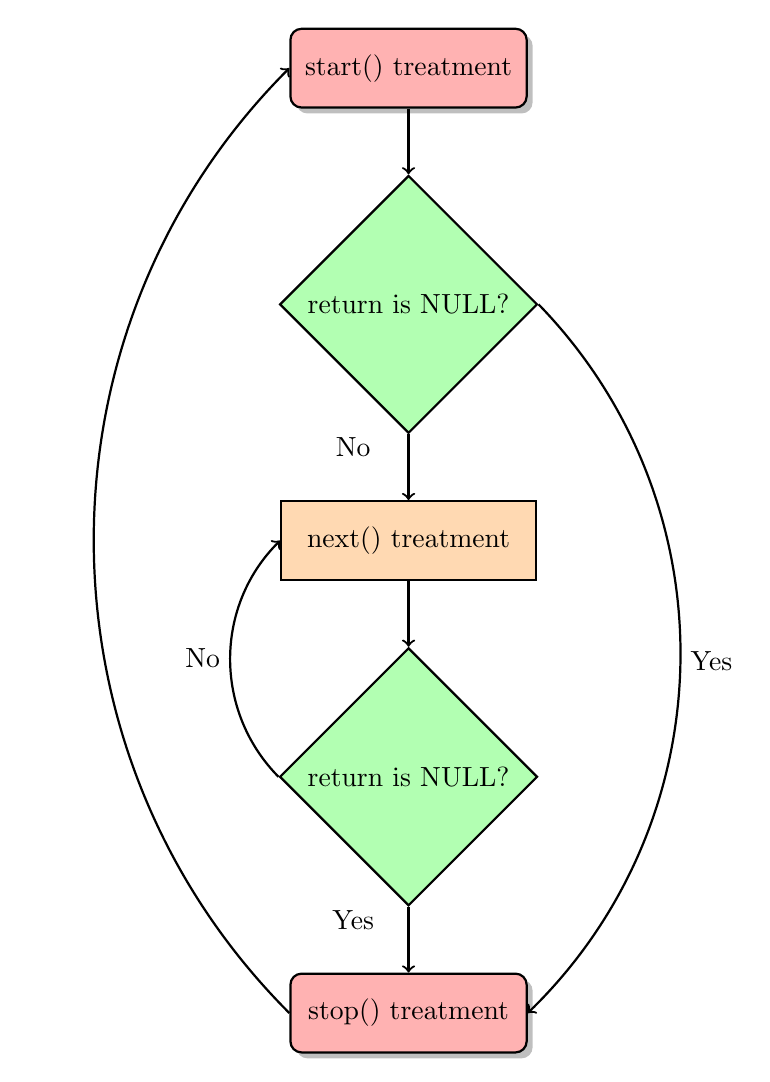
\begin{tikzpicture}[node distance=2cm, thick]
    \node (start) [startstop] {start() treatment};
    \node (branch1) [decision, below of=start, yshift=-1cm] {return is NULL?};
    \node (next) [process, below of=branch1, yshift=-1cm] {next() treatment};
    \node (branch2) [decision, below of=next, yshift=-1cm] {return is NULL?};
    \node (stop) [startstop, below of=branch2, yshift=-1cm] {stop() treatment};

    \draw [->] (start) -- (branch1);
    \draw [->] (branch1.east) to [out=135, in=-135, bend left=45] node [right] {Yes} (stop.east);
    \draw [->] (branch1) -- node[left=2em, anchor=south] {No} (next);
    \draw [->] (next) -- (branch2);
    \draw [->] (branch2.west) to [out=135, in=-135, bend left=45] node [left] {No} (next.west);
    \draw [->] (branch2) -- node[left=2em, anchor=south] {Yes} (stop);
    \draw [->] (stop.west) to [out=135, in=-135] node [left] {} (start.west);
  \end{tikzpicture}
  \caption{How seq\_file works}
  \label{img:seqfile}
\end{figure}

The \cpp|seq_file| provides basic functions for \cpp|proc_ops|, such as \cpp|seq_read|, \cpp|seq_lseek|, and some others.
But nothing to write in the \verb|/proc| file.
Of course, you can still use the same way as in the previous example.

\samplec{examples/procfs4.c}

If you want more information, you can read this web page:

\begin{itemize}
  \item \url{https://lwn.net/Articles/22355/}
  \item \url{https://kernelnewbies.org/Documents/SeqFileHowTo}
\end{itemize}

You can also read the code of \src{fs/seq\_file.c} in the Linux kernel.

\section{sysfs: Interacting with your module}
\label{sec:sysfs}
\emph{sysfs} allows you to interact with the running kernel from userspace by reading or setting variables inside of modules.
This can be useful for debugging purposes, or just as an interface for applications or scripts.
You can find sysfs directories and files under the \verb|/sys| directory on your system.

\begin{codebash}
ls -l /sys
\end{codebash}

Unlike \verb|/proc|, which grew organically and mixes process information with driver knobs, sysfs is tightly tied to the kernel's device model and provides multiple coherent views of the same hardware:

\begin{itemize}
  \item \verb|/sys/devices/|: the actual device tree, rooted at the platform/CPU level.
  \item \verb|/sys/bus/|: one subdirectory per bus type (PCI, USB, I2C, platform, \dots), each containing \verb|devices/| and \verb|drivers/| subdirectories. Entries under \verb|devices/| are symlinks back into \verb|/sys/devices/|.
  \item \verb|/sys/class/|: devices grouped by function (net, block, input, tty, \dots) regardless of what bus they sit on.
  \item \verb|/sys/module/|: one directory per module (including built-in ones), exposing parameters and, for loadable modules, reference count.
  \item \verb|/sys/kernel/|: miscellaneous kernel-wide tunables.
  \item \verb|/sys/firmware/|: firmware and ACPI/device-tree data.
  \item \verb|/sys/power/|: power-management state.
\end{itemize}

Every directory in sysfs corresponds to a \cpp|struct kobject| in the kernel.
Files inside those directories are kobject attributes; read or write operations on them invoke \cpp|show()| or \cpp|store()| callbacks inside the driver.
This one-value-per-file convention keeps the interface simple and scriptable compared to the free-form output of many \verb|/proc| entries.

Attributes can be exported for kobjects in the form of regular files in the filesystem.
Sysfs forwards file I/O operations to methods defined for the attributes, providing a means to read and write kernel attributes.

A simple attribute definition:

\begin{code}
struct attribute {
    char *name;
    struct module *owner;
    umode_t mode;
};

int sysfs_create_file(struct kobject * kobj, const struct attribute * attr);
void sysfs_remove_file(struct kobject * kobj, const struct attribute * attr);
\end{code}

For example, the driver model defines \cpp|struct device_attribute| like:

\begin{code}
struct device_attribute {
    struct attribute attr;
    ssize_t (*show)(struct device *dev, struct device_attribute *attr,
                    char *buf);
    ssize_t (*store)(struct device *dev, struct device_attribute *attr,
                    const char *buf, size_t count);
};

int device_create_file(struct device *, const struct device_attribute *);
void device_remove_file(struct device *, const struct device_attribute *);
\end{code}

To read or write attributes, the \cpp|show()| or \cpp|store()| method must be specified when declaring the attribute.
For the common cases \src{include/linux/sysfs.h} provides convenience macros (\cpp|__ATTR|, \cpp|__ATTR_RO|, \cpp|__ATTR_WO|, etc.) to make defining attributes easier as well as making code more concise and readable.

An example of a hello world module which includes the creation of a variable accessible via sysfs is given below.

\samplec{examples/hello-sysfs.c}

Make and install the module:

\begin{codebash}
make
sudo insmod hello-sysfs.ko
\end{codebash}

Check that it exists:

\begin{codebash}
lsmod | grep hello_sysfs
\end{codebash}

What is the current value of \cpp|myvariable| ?

\begin{codebash}
cat /sys/kernel/mymodule/myvariable
\end{codebash}

Set the value of \cpp|myvariable| and check that it changed.

\begin{codebash}
echo "32" | sudo tee /sys/kernel/mymodule/myvariable
cat /sys/kernel/mymodule/myvariable
\end{codebash}

Finally, remove the test module:

\begin{codebash}
sudo rmmod hello_sysfs
\end{codebash}

In the above case, we use a simple kobject to create a directory under sysfs, and communicate with its attributes.
Since Linux v2.6.0, the \cpp|kobject| structure made its appearance.
It was initially meant as a simple way of unifying kernel code which manages reference counted objects.
After a bit of mission creep, it is now the glue that holds much of the device model and its sysfs interface together.
For more information about kobject and sysfs, see \src{Documentation/driver-api/driver-model/driver.rst} and \url{https://lwn.net/Articles/51437/}.

\section{debugfs: Flexible debugging interfaces}
\label{sec:debugfs}
\emph{debugfs} is a lightweight filesystem for exporting debugging information from the kernel to userspace.
Unlike \verb|sysfs|, it is not intended to provide a stable userspace ABI, and unlike \verb|/proc| it does not try to model processes or broader kernel state.
That makes it a good fit for ad hoc diagnostics, counters, and developer-oriented control points while a module is under active development.

The canonical introduction is \src{Documentation/filesystems/debugfs.rst}, which describes both the design goals and the helper APIs.
On most systems, debugfs is mounted at \verb|/sys/kernel/debug|:

\begin{codebash}
mount | grep debugfs
ls -l /sys/kernel/debug
\end{codebash}

To use the interface, include \src{include/linux/debugfs.h} and create a top-level directory for your module:

\begin{code}
struct dentry *debugfs_create_dir(const char *name, struct dentry *parent);
\end{code}

Passing \cpp|NULL| as the parent places the new directory at the root of debugfs.
When you unload the module, remove the whole subtree with \cpp|debugfs_remove_recursive()|.
Note that \cpp|debugfs_create_dir()| and the other \verb|debugfs_create_*()| helpers are designed to be used in a fire-and-forget fashion: their return values should not be checked.
If debugfs is unavailable or an entry cannot be created, the helpers return an error pointer that is silently accepted by subsequent calls and by \cpp|debugfs_remove_recursive()|, so the module continues to work without its debug interface.

For simple scalar values, debugfs provides typed helpers that map a kernel variable directly to a file.
Common examples include \cpp|debugfs_create_u32()|, \cpp|debugfs_create_bool()|, and the hexadecimal variants such as \cpp|debugfs_create_x32()|.
These helpers are convenient when the data already lives in a fixed-size variable and does not need custom formatting.

The following example creates a debugfs directory and exports a writable integer plus a boolean flag:

\samplec{examples/hello-debugfs.c}

If you need a custom text format or more control over reads and writes, create a file with your own \cpp|struct file_operations|:

\begin{code}
struct dentry *debugfs_create_file(const char *name, umode_t mode,
                                   struct dentry *parent, void *data,
                                   const struct file_operations *fops);
\end{code}

debugfs also includes helpers for a few common read-only payloads.
One of them is \cpp|debugfs_create_blob()|, which exposes an existing memory region as a file.

The next example combines both approaches by creating a writable debugfs file and a read-only blob in the same directory:

\samplec{examples/hello-debugfs-file.c}

Because debugfs is explicitly for debugging, its contents should be treated as implementation details rather than a supported external interface.
If a setting must remain stable for tooling, scripts, or end users, prefer \verb|sysfs| or another documented ABI instead.

\section{Talking To Device Files}
\label{sec:device_files}
Device files are supposed to represent physical devices.
Most physical devices are used for output as well as input, so there has to be some mechanism for device drivers in the kernel to get the output to send to the device from processes.
This is done by opening the device file for output and writing to it, just like writing to a file.
In the following example, this is implemented by \cpp|device_write|.

This is not always enough.
Imagine you had a serial port connected to a modem (even if you have an internal modem, it is still implemented from the CPU's perspective as a serial port connected to a modem, so you don't have to tax your imagination too hard).
The natural thing to do would be to use the device file to write things to the modem (either modem commands or data to be sent through the phone line) and read things from the modem (either responses for commands or the data received through the phone line).
However, this leaves open the question of what to do when you need to talk to the serial port itself, for example to configure the rate at which data is sent and received.

The answer in Unix is to use a special function called \cpp|ioctl| (short for Input Output ConTroL).
Every device can have its own \cpp|ioctl| commands, which can be read ioctl operations (to send information from a process to the kernel), write ioctl operations (to return information to a process), both or neither.
Notice here the roles of read and write are reversed again, so in ioctl operations, read is to send information to the kernel and write is to receive information from the kernel.

The ioctl function is called with three parameters: the file descriptor of the appropriate device file, the ioctl number, and a parameter, which is of type long so you can use a cast to use it to pass anything.
You will not be able to pass a structure this way, but you will be able to pass a pointer to the structure.
Here is an example:

\samplec{examples/ioctl.c}

You can see there is an argument called \cpp|cmd| in \cpp|test_ioctl_ioctl()| function.
It is the ioctl number.
The ioctl number encodes the major device number, the type of the ioctl, the command, and the type of the parameter.
This ioctl number is usually created by a macro call (\cpp|_IO|, \cpp|_IOR|, \cpp|_IOW| or \cpp|_IOWR| --- depending on the type) in a header file.
This header file should then be included both by the programs which will use ioctl (so they can generate the appropriate ioctl operations) and by the kernel module (so it can understand it).
In the example below, the header file is \verb|chardev.h| and the program which uses it is \verb|userspace_ioctl.c|.

If you want to use ioctls in your own kernel modules, it is best to receive an official ioctl assignment, so if you accidentally get somebody else's ioctls, or if they get yours, you'll know something is wrong.
For more information, consult the kernel source tree at \src{Documentation/userspace-api/ioctl/ioctl-number.rst}.

Also, we need to be careful that concurrent access to the shared resources will lead to the race condition.
The solution is using atomic Compare-And-Swap (CAS), which we mentioned at \Cref{sec:chardev_c}, to enforce the exclusive access.

\samplec{examples/chardev2.c}

\samplec{examples/chardev.h}

\samplec{examples/other/userspace_ioctl.c}

\subsection{poll, select, and epoll}
\label{sec:poll_select_epoll}
The traditional \cpp|read()| and \cpp|write()| paths are not enough for every
character device.
Many programs need to wait on multiple file descriptors at once, and for that
they use \cpp|poll()|, \cpp|select()|, or most commonly \cpp|epoll|.
If a driver can block in \cpp|read()| or \cpp|write()|, it usually also needs a
\cpp|poll| callback so userspace can discover when the operation would make
progress without spinning.

The kernel-side implementation is centered on the \cpp|poll| file operation.
The callback receives a \cpp|poll_table_struct|, and the usual pattern is to
register the caller with one or more wait queues using \cpp|poll_wait()| before
computing the readiness mask to return.
That mask is built from \cpp|EPOLLIN|, \cpp|EPOLLOUT|, \cpp|EPOLLERR|,
\cpp|EPOLLHUP|, and related bits.
The names still mention epoll, but the same mask is used by \cpp|poll()| and
\cpp|select()|.

Correct readiness reporting matters because modern event loops often rely on
edge-triggered epoll.
If a driver returns readable status without guaranteeing that a subsequent
\cpp|read()| can consume data, or forgets to wake waiters after state changes,
userspace can wedge in hard-to-debug ways.
Likewise, returning \cpp|EPOLLHUP| or \cpp|EPOLLERR| too eagerly can make a
device appear permanently dead.
The rule of thumb is simple: the mask should describe what a nonblocking call
would be able to do \emph{right now}.

When device state changes, wake the relevant wait queue.
If you want fine-grained wakeups, use \cpp|wake_up_interruptible_poll()| with
the same event bits your \cpp|poll| callback reports.
That allows userspace to sleep efficiently until the device becomes readable,
writable, or otherwise transitions into a new state.

The sleep example in \Cref{sec:sleep} already demonstrates the wait-queue side
of blocking I/O.
Adding \cpp|poll| support to a driver is mostly a matter of exposing that same
state transition to event-driven applications instead of forcing them to block
in one system call at a time.

\subsection{Asynchronous notification}
\label{sec:async_notification}
Another classic mechanism described in LDD3 is asynchronous notification via
\cpp|SIGIO|.
This is implemented with the \cpp|fasync| file operation and helpers such as
\cpp|fasync_helper()| and \cpp|kill_fasync()|.
When enabled from userspace with \cpp|fcntl(F\_SETFL, O\_ASYNC)|, the process
receives a signal when the device becomes ready.

This interface still exists in Linux 5.10 and later, but it is much less common than
\cpp|poll| and epoll-based designs.
Signals are process-directed, relatively coarse, and awkward in multithreaded
programs.
For new user interfaces, a well-behaved \cpp|poll| implementation is usually
the better default.
Still, \cpp|fasync| remains useful for compatibility with older applications or
for small control-style devices that only need to notify userspace that some
event happened.

\chapter{Execution Context and Control Flow}
Kernel code runs under a variety of constraints depending on where it executes.
Some paths may sleep, some must return quickly, and some need careful
synchronization to stay correct on modern SMP systems. This chapter collects
the mechanisms that shape control flow, blocking behavior, deferred work, and
debugging.

\section{System Calls}
\label{sec:syscall}
So far, the only thing we've done was to use well defined kernel mechanisms to register \verb|/proc| files and device handlers.
This is fine if you want to do something the kernel programmers thought you'd want, such as write a device driver.
But what if you want to do something unusual, to change the behavior of the system in some way?
Then, you are mostly on your own.

Notice that this example has been unavailable since Linux v6.9.
Specifically, after this \href{https://github.com/torvalds/linux/commit/1e3ad78334a69b36e107232e337f9d693dcc9df2#diff-4a16bf89a09b4f49669a30d54540f0b936ea0224dc6ee9edfa7700deb16c3e11R52}{commit}, due to the system call table changing the implementation from an indirect function call table to a switch statement for security issues, such as Branch History Injection (BHI) attack.
See more information \href{https://bugs.launchpad.net/ubuntu/+source/linux/+bug/2060909}{here}.

Should one choose not to use a virtual machine, kernel programming can become risky.
For example, while writing the code below, the \cpp|open()| system call was inadvertently disrupted.
This resulted in an inability to open any files, run programs, or shut down the system, necessitating a restart of the virtual machine.
Fortunately, no critical files were lost in this instance.
However, if such modifications were made on a live, mission-critical system, the consequences could be severe.
To mitigate the risk of file loss, even in a test environment, it is advised to execute \sh|sync| right before using \sh|insmod| and \sh|rmmod|.

Forget about \verb|/proc| files, forget about device files.
They are just minor details.
Minutiae in the vast expanse of the universe.
The real process to kernel communication mechanism, the one used by all processes, is \emph{system calls}.
When a process requests a service from the kernel (such as opening a file, forking to a new process, or requesting more memory), this is the mechanism used.
If you want to change the behaviour of the kernel in interesting ways, this is the place to do it.
By the way, if you want to see which system calls a program uses, run \sh|strace <arguments>|.

In general, a process is not supposed to be able to access the kernel.
It can not access kernel memory and it can't call kernel functions.
The hardware of the CPU enforces this (that is the reason why it is called ``protected mode'' or ``page protection'').

System calls are an exception to this general rule.
What happens is that the process fills the registers with the appropriate values and then calls a special instruction which jumps to a previously defined location in the kernel (of course, that location is readable by user processes, it is not writable by them).
Under Intel CPUs, this is done by means of interrupt 0x80. The hardware knows that once you jump to this location, you are no longer running in restricted user mode, but as the operating system kernel --- and therefore you're allowed to do whatever you want.

% FIXME: recent kernel changes the system call entries
The location in the kernel a process can jump to is called \verb|system_call|.
The procedure at that location checks the system call number, which tells the kernel what service the process requested.
Then, it looks at the table of system calls (\cpp|sys_call_table|) to see the address of the kernel function to call.
Then it calls the function, and after it returns, does a few system checks and then return back to the process (or to a different process, if the process time ran out).
If you want to read this code, it is at the source file \verb|arch/$(architecture)/kernel/entry.S|, after the line \cpp|ENTRY(system_call)|.

So, if we want to change the way a certain system call works, what we need to do is to write our own function to implement it (usually by adding a bit of our own code, and then calling the original function) and then change the pointer at \cpp|sys_call_table| to point to our function.
Because we might be removed later and we don't want to leave the system in an unstable state, it's important for \cpp|cleanup_module| to restore the table to its original state.

To modify the content of \cpp|sys_call_table|, we need to consider the control register.
A control register is a processor register that changes or controls the general behavior of the CPU.
For x86 architecture, the \verb|cr0| register has various control flags that modify the basic operation of the processor.
The \verb|WP| flag in \verb|cr0| stands for write protection.
Once the \verb|WP| flag is set, the processor disallows further write attempts to the read-only sections.
Therefore, we must disable the \verb|WP| flag before modifying \cpp|sys_call_table|.
Since Linux v5.3, the \cpp|write_cr0| function cannot be used because of the sensitive \verb|cr0| bits pinned by the security issue, the attacker may write into CPU control registers to disable CPU protections like write protection.
As a result, we have to provide the custom assembly routine to bypass it.

However, \cpp|sys_call_table| symbol is unexported to prevent misuse.
But there have few ways to get the symbol, manual symbol lookup and \cpp|kallsyms_lookup_name|.
Here we use both depend on the kernel version.

Because of the \textit{control-flow integrity}, which is a technique to prevent the redirect execution code from the attacker, for making sure that the indirect calls go to the expected addresses and the return addresses are not changed.
Since Linux v5.7, the kernel patched the series of \textit{control-flow enforcement} (CET) for x86,
and some configurations of GCC, like GCC versions 9 and 10 in Ubuntu Linux,
will add with CET (the \verb|-fcf-protection| option) in the kernel by default.
Using that GCC to compile the kernel with retpoline off may result in CET being enabled in the kernel.
You can use the following command to check out the \verb|-fcf-protection| option is enabled or not:
\begin{verbatim}
$ gcc -v -Q -O2 --help=target | grep protection
Using built-in specs.
COLLECT_GCC=gcc
COLLECT_LTO_WRAPPER=/usr/lib/gcc/x86_64-linux-gnu/9/lto-wrapper
...
gcc version 9.3.0 (Ubuntu 9.3.0-17ubuntu1~20.04)
COLLECT_GCC_OPTIONS='-v' '-Q' '-O2' '--help=target' '-mtune=generic' '-march=x86-64'
 /usr/lib/gcc/x86_64-linux-gnu/9/cc1 -v ... -fcf-protection ...
 GNU C17 (Ubuntu 9.3.0-17ubuntu1~20.04) version 9.3.0 (x86_64-linux-gnu)
...
\end{verbatim}
But CET should not be enabled in the kernel, it may break the Kprobes and bpf.
Consequently, CET is disabled since v5.11.
To guarantee the manual symbol lookup worked, we only use up to v5.4.

Unfortunately, since Linux v5.7 \cpp|kallsyms_lookup_name| is also unexported, it needs certain trick to get the address of \cpp|kallsyms_lookup_name|.
If \cpp|CONFIG_KPROBES| is enabled, we can facilitate the retrieval of function addresses by means of Kprobes to dynamically break into the specific kernel routine.
Kprobes inserts a breakpoint at the entry of function by replacing the first bytes of the probed instruction.
When a CPU hits the breakpoint, registers are stored, and the control will pass to Kprobes.
It passes the addresses of the saved registers and the Kprobe struct to the handler you defined, then executes it.
Kprobes can be registered by symbol name or address.
Within the symbol name, the address will be handled by the kernel.

Otherwise, specify the address of \cpp|sys_call_table| from \verb|/proc/kallsyms| and \verb|/boot/System.map| into \cpp|sym| parameter.
Following is the sample usage for \verb|/proc/kallsyms|:
\begin{verbatim}
$ sudo grep sys_call_table /proc/kallsyms
ffffffff82000280 R x32_sys_call_table
ffffffff820013a0 R sys_call_table
ffffffff820023e0 R ia32_sys_call_table
$ sudo insmod syscall-steal.ko sym=0xffffffff820013a0
\end{verbatim}

Using the address from \verb|/boot/System.map|, be careful about \verb|KASLR| (Kernel Address Space Layout Randomization).
\verb|KASLR| may randomize the address of kernel code and data at every boot time, such as the static address listed in \verb|/boot/System.map| will offset by some entropy.
The purpose of \verb|KASLR| is to protect the kernel space from the attacker.
Without \verb|KASLR|, the attacker may find the target address in the fixed address easily.
Then the attacker can use return-oriented programming to insert some malicious codes to execute or receive the target data by a tampered pointer.
\verb|KASLR| mitigates these kinds of attacks because the attacker cannot immediately know the target address, but a brute-force attack can still work.
If the address of a symbol in \verb|/proc/kallsyms| is different from the address in \verb|/boot/System.map|, \verb|KASLR| is enabled with the kernel, on which your system is running.
\begin{verbatim}
$ grep GRUB_CMDLINE_LINUX_DEFAULT /etc/default/grub
GRUB_CMDLINE_LINUX_DEFAULT="quiet splash"
$ sudo grep sys_call_table /boot/System.map-$(uname -r)
ffffffff82000300 R sys_call_table
$ sudo grep sys_call_table /proc/kallsyms
ffffffff820013a0 R sys_call_table
# Reboot
$ sudo grep sys_call_table /boot/System.map-$(uname -r)
ffffffff82000300 R sys_call_table
$ sudo grep sys_call_table /proc/kallsyms
ffffffff86400300 R sys_call_table
\end{verbatim}
If \verb|KASLR| is enabled, we have to take care of the address from \verb|/proc/kallsyms| each time we reboot the machine.
In order to use the address from \verb|/boot/System.map|, make sure that \verb|KASLR| is disabled.
You can add the \verb|nokaslr| for disabling \verb|KASLR| in next booting time:
\begin{verbatim}
$ grep GRUB_CMDLINE_LINUX_DEFAULT /etc/default/grub
GRUB_CMDLINE_LINUX_DEFAULT="quiet splash"
$ sudo perl -i -pe 'm/quiet/ and s//quiet nokaslr/' /etc/default/grub
$ grep quiet /etc/default/grub
GRUB_CMDLINE_LINUX_DEFAULT="quiet nokaslr splash"
$ sudo update-grub
\end{verbatim}

For more information, check out the following:

\begin{itemize}
  \item \href{https://lwn.net/Articles/804849/}{Cook: Security things in Linux v5.3}
  \item \href{https://lwn.net/Articles/12211/}{Unexporting the system call table}
  \item \href{https://lwn.net/Articles/810077/}{Control-flow integrity for the kernel}
  \item \href{https://lwn.net/Articles/813350/}{Unexporting kallsyms\_lookup\_name()}
  \item \href{https://www.kernel.org/doc/Documentation/kprobes.txt}{Kernel Probes (Kprobes)}
  \item \href{https://lwn.net/Articles/569635/}{Kernel address space layout randomization}
\end{itemize}

The source code here is an example of such a kernel module.
We want to ``spy'' on a certain user, and to \cpp|pr_info()| a message whenever that user opens a file.
Towards this end, we replace the system call to open a file with our own function, called \cpp|our_sys_openat|.
This function checks the uid (user's id) of the current process, and if it is equal to the uid we spy on, it calls \cpp|pr_info()| to display the name of the file to be opened.
Then, either way, it calls the original \cpp|openat()| function with the same parameters, to actually open the file.

The \cpp|init_module| function replaces the appropriate location in \cpp|sys_call_table| and keeps the original pointer in a variable.
The \cpp|cleanup_module| function uses that variable to restore everything back to normal.
This approach is dangerous, because of the possibility of two kernel modules changing the same system call.
Imagine we have two kernel modules, A and B. A's openat system call will be \cpp|A_openat| and B's will be \cpp|B_openat|.
Now, when A is inserted into the kernel, the system call is replaced with \cpp|A_openat|, which will call the original \cpp|sys_openat| when it is done.
Next, B is inserted into the kernel, which replaces the system call with \cpp|B_openat|, which will call what it thinks is the original system call, \cpp|A_openat|, when it's done.

Now, if B is removed first, everything will be well --- it will simply restore the system call to \cpp|A_openat|, which calls the original.
However, if A is removed and then B is removed, the system will crash.
A's removal will restore the system call to the original, \cpp|sys_openat|, cutting B out of the loop.
Then, when B is removed, it will restore the system call to what it thinks is the original, \cpp|A_openat|, which is no longer in memory.
At first glance, it appears we could solve this particular problem by checking if the system call is equal to our open function and if so not changing it at all (so that B won't change the system call when it is removed), but that will cause an even worse problem.
When A is removed, it sees that the system call was changed to \cpp|B_openat| so that it is no longer pointing to \cpp|A_openat|, so it will not restore it to \cpp|sys_openat| before it is removed from memory.
Unfortunately, \cpp|B_openat| will still try to call \cpp|A_openat| which is no longer there, so that even without removing B the system would crash.

For x86 architecture, the system call table cannot be used to invoke a system call after commit
\href{https://git.kernel.org/pub/scm/linux/kernel/git/torvalds/linux.git/commit/?id=1e3ad78334a69b36e107232e337f9d693dcc9df2}{1e3ad78} since v6.9.
This commit has been backported to long term stable kernels, like v5.15.154+, v6.1.85+, v6.6.26+ and v6.8.5+, see this \href{https://stackoverflow.com/a/78607015}{answer} for more details.
In this case, thanks to Kprobes, a hook can be used instead on the system call entry to intercept the system call.

Note that all the related problems make syscall stealing unfeasible for production use.
In order to keep people from doing potentially harmful things \cpp|sys_call_table| is no longer exported.
This means, if you want to do something more than a mere dry run of this example, you will have to patch your current kernel in order to have \cpp|sys_call_table| exported.

\samplec{examples/syscall-steal.c}

\section{Blocking Processes and threads}
\label{sec:blocking_process_thread}
\subsection{Sleep}
\label{sec:sleep}
What do you do when somebody asks you for something you can not do right away?
If you are a human being and you are bothered by a human being, the only thing you can say is: "\emph{Not right now, I'm busy. Go away!}".
But if you are a kernel module and you are bothered by a process, you have another possibility.
You can put the process to sleep until you can service it.
After all, processes are being put to sleep by the kernel and woken up all the time (that is the way multiple processes appear to run on the same time on a single CPU).

This kernel module is an example of this.
The file (called \verb|/proc/sleep|) can only be opened by a single process at a time.
If the file is already open, the kernel module calls \cpp|wait_event_interruptible|.
The easiest way to keep a file open is to open it with:

\begin{codebash}
tail -f
\end{codebash}

This function changes the status of the task (a task is the kernel data structure which holds information about a process and the system call it is in,
if any) to \cpp|TASK_INTERRUPTIBLE|, which means that the task will not run until it is woken up somehow, and adds it to WaitQ, the queue of tasks waiting to access the file.
Then, the function calls the scheduler to context switch to a different process, one which has some use for the CPU.

When a process is done with the file, it closes it, and \cpp|module_close| is called.
That function wakes up all the processes in the queue (there's no mechanism to only wake up one of them).
It then returns and the process which just closed the file can continue to run.
In time, the scheduler decides that that process has had enough and gives control of the CPU to another process.
Eventually, one of the processes which was in the queue will be given control of the CPU by the scheduler.
It starts at the point right after the call to \cpp|wait_event_interruptible|.

This means that the process is still in kernel mode - as far as the process is concerned, it issued the open system call and the system call has not returned yet.
The process does not know somebody else used the CPU for most of the time between the moment it issued the call and the moment it returned.

It can then proceed to set a global variable to tell all the other processes that the file is still open and go on with its life.
When the other processes get a piece of the CPU, they'll see that global variable and go back to sleep.

So we will use \sh|tail -f| to keep the file open in the background, and attempt to access it with another background process.
This way, we don't need to switch to another terminal window or virtual terminal to run the second process.
As soon as the first background process is killed with kill \%1 , the second is woken up, is able to access the file and finally terminates.

To make our life more interesting, \cpp|module_close| does not have a monopoly on waking up the processes which wait to access the file.
A signal, such as \emph{Ctrl +c} (\textbf{SIGINT}) can also wake up a process. This is because we used \cpp|wait_event_interruptible|.
We could have used \cpp|wait_event| instead, but that would have resulted in extremely angry users whose \emph{Ctrl+c}'s are ignored.

In that case, we want to return with \cpp|-EINTR| immediately. This is important so users can, for example, kill the process before it receives the file.

There is one more point to remember. Some times processes don't want to sleep, they want either to get what they want immediately, or to be told it cannot be done.
Such processes use the \cpp|O_NONBLOCK| flag when opening the file.
The kernel is supposed to respond by returning with the error code \cpp|-EAGAIN| from operations which would otherwise block, such as opening the file in this example. The program \sh|cat_nonblock|, available in the \verb|examples/other| directory, can be used to open a file with \cpp|O_NONBLOCK|.

\begin{verbatim}
$ sudo insmod sleep.ko
$ cat_nonblock /proc/sleep
Last input:
$ tail -f /proc/sleep &
Last input:
Last input:
Last input:
Last input:
Last input:
Last input:
Last input:
tail: /proc/sleep: file truncated
[1] 6540
$ cat_nonblock /proc/sleep
Open would block
$ kill %1
[1]+  Terminated              tail -f /proc/sleep
$ cat_nonblock /proc/sleep
Last input:
$
\end{verbatim}

\samplec{examples/sleep.c}

\samplec{examples/other/cat_nonblock.c}

\subsection{Completions}
\label{sec:completion}
Sometimes one thing should happen before another within a module having multiple threads.
Rather than using \sh|/bin/sleep| commands, the kernel has another way to do this which allows timeouts or interrupts to also happen.

Completions as code synchronization mechanism have three main parts, initialization of struct completion synchronization object, the waiting or barrier part through \cpp|wait_for_completion()|, and the signalling side through a call to \cpp|complete()|.

In the subsequent example, two threads are initiated: crank and flywheel.
It is imperative that the crank thread starts before the flywheel thread.
A completion state is established for each of these threads, with a distinct completion defined for both the crank and flywheel threads.
At the exit point of each thread the respective completion state is updated, and \cpp|wait_for_completion| is used by the flywheel thread to ensure that it does not begin prematurely.
The crank thread uses the \cpp|complete_all()| function to update the completion, which lets the flywheel thread continue.

So even though \cpp|flywheel_thread| is started first you should notice when you load this module and run \sh|dmesg|, that turning the crank always happens first because the flywheel thread waits for the crank thread to complete.

There are other variations of the \cpp|wait_for_completion| function, which include timeouts or being interrupted, but this basic mechanism is enough for many common situations without adding a lot of complexity.

\samplec{examples/completions.c}

\section{Synchronization}
\label{sec:synchronization}
If processes running on different CPUs or in different threads try to access the same memory, then it is possible that strange things can happen or your system can lock up.
To avoid this, various types of mutual exclusion kernel functions are available.
These indicate if a section of code is "locked" or "unlocked" so that simultaneous attempts to run it can not happen.
\subsection{Mutex}
\label{sec:mutex}
You can use kernel mutexes (mutual exclusions) in much the same manner that you might deploy them in userland.
This may be all that is needed to avoid collisions in most cases.

Mutexes in the Linux kernel enforce strict ownership: only the task that successfully acquired the mutex can release (or unlock) it.
Attempting to release a mutex held by another task or releasing an unheld mutex multiple times by the same task typically leads to errors or undefined behavior.
If a task tries to lock a mutex it already holds, it may be blocked or sleep, where the task waits for itself to release the lock.

Before use, a mutex must be initialized through specific APIs (such as \cpp|mutex_init| or by using the \cpp|DEFINE_MUTEX| macro for compile-time initialization).
And it is prohibited to directly modify the internal structure of a mutex using a memory manipulation function like \cpp|memset|.

\samplec{examples/example_mutex.c}

The various suffixes appended to mutex functions in the Linux kernel primarily dictate how a task waiting to acquire a lock will behave,
particularly concerning its interruptibility.

When a task calls \cpp|mutex_lock()|, and if the mutex is currently unavailable,
the task enters a sleep state until it can successfully obtain the lock.
During this period, the task cannot be interrupted.
In contrast, functions with the \cpp|_interruptible| suffix, such as \cpp|mutex_lock_interruptible()|,
behave similarly to \cpp|mutex_lock()| but allow the waiting process to be interrupted by signals.
If a task receives a signal (like a termination signal) while waiting for the lock,
it will exit the waiting state and return an error code (\cpp|-EINTR|).
This is useful for applications that need to handle external events even while waiting for a lock.

Beyond these fundamental locking behaviors, other mutex functions offer specialized capabilities.
Functions like \cpp|mutex_lock_nested| and \cpp|mutex_lock_interruptible_nested()| incorporate the \cpp|__nested()| functionality,
providing support for nested locking.
This prior locking mechanism aids in managing lock acquisition and preventing deadlocks,
often employing a subclass parameter for more precise deadlock detection.
The latter variant combines nested locking with the ability for the waiting process to be interrupted by signals.
Another function is \cpp|mutex_trylock()|, which attempts to acquire the mutex without blocking.
It returns 1 if the lock is successfully acquired and 0 if the mutex is already held by another task.

Despite the fact that \cpp|mutex_trylock| does not sleep,
it is still generally not safe for use in interrupt context because its implementation isn't atomic.
If an interrupt occurs between checking the lock's availability and its acquisition,
this can lead to race conditions and potential data corruption.

\subsection{Spinlocks}
\label{sec:spinlock}
As the name suggests, spinlocks lock up the CPU that the code is running on, taking 100\% of its resources.
Because of this you should only use the spinlock mechanism around code which is likely to take no more than a few milliseconds to run and so will not noticeably slow anything down from the user's point of view.

The example here is \verb|"irq safe"| in that if interrupts happen during the lock then they will not be forgotten and will activate when the unlock happens, using the \cpp|flags| variable to retain their state.

\samplec{examples/example_spinlock.c}

Taking 100\% of a CPU's resources comes with greater responsibility.
Situations where the kernel code monopolizes a CPU are called \textbf{atomic contexts}.
Holding a spinlock is one of those situations.
Sleeping in atomic contexts may leave the system hanging, as the occupied CPU devotes 100\% of its resources doing nothing but sleeping.
In some worse cases the system may crash.
Thus, sleeping in atomic contexts is considered a bug in the kernel.
They are sometimes called ``sleep-in-atomic-context'' in some materials.

Note that sleeping here is not limited to calling the sleep functions explicitly.
If subsequent function calls eventually invoke a function that sleeps, it is also considered sleeping.
Thus, it is important to pay attention to functions being used in atomic context.
There's no documentation recording all such functions, but code comments may help.
Sometimes you may find comments in kernel source code stating that a function ``may sleep'', ``might sleep'', or more explicitly ``the caller should not hold a spinlock''.
Those comments are hints that a function may implicitly sleep and must not be called in atomic contexts.

Now, let's differentiate between a few types of spinlock functions in the Linux kernel: \cpp|spin_lock()|, \cpp|spin_lock_irq()|, \cpp|spin_lock_irqsave()|, and \cpp|spin_lock_bh()|.

\cpp|spin_lock()| does not allow the CPU to sleep while waiting for the lock, which makes it suitable for most use cases where the critical section is short.
However, this is problematic for real-time Linux because spinlocks in this configuration behave as sleeping locks.
This can prevent other tasks from running and cause the system to become unresponsive.
To address this in real-time Linux environments, a \cpp|raw_spin_lock()| is used, which behaves similarly to a \cpp|spin_lock()| but without causing the system to sleep.

On non-\verb|PREEMPT_RT| kernels, \cpp|spin_lock_irq()| disables local hard interrupts before acquiring the lock, and \cpp|spin_unlock_irq()| unconditionally re-enables them when the lock is released.
Because this pair does not save the previous interrupt state, use it only when you know hard interrupts are enabled on entry and it is correct to re-enable them on exit.
In contrast, \cpp|spin_lock_irqsave()| disables local hard interrupts and stores the previous state in an opaque \cpp|unsigned long flags| variable.
The matching \cpp|spin_unlock_irqrestore()| restores that saved state, so it is safe regardless of whether hard interrupts were enabled or disabled before entering the critical section.
This makes \cpp|spin_lock_irqsave()| the preferred interface when a function may be called from both process context and hardirq context, or from any path where the caller's interrupt state is unknown.
On \verb|PREEMPT_RT| kernels, \cpp|spinlock_t| becomes an RT-mutex-based sleeping lock, so the \cpp|_irq| and \cpp|_irqsave| suffixes do not actually disable hardware interrupts.
If you genuinely need hard interrupts disabled, use the \cpp|raw_spin_lock_irqsave()| family (see \cpp|raw_spin_lock()| above), but note that raw spinlocks really spin, disable preemption, and must not be held across any potentially sleeping operation.

Next, \cpp|spin_lock_bh()| disables \textbf{softirqs} (software interrupts) but allows hardware interrupts to continue.
Unlike \cpp|spin_lock_irq()| and \cpp|spin_lock_irqsave()|, which disable both hardware and software interrupts, \cpp|spin_lock_bh()| is useful when hardware interrupts need to remain active.

A common deadlock scenario illustrates why the right variant matters.
Suppose process-context code acquires a spinlock with plain \cpp|spin_lock()|, then a hardware interrupt fires on the same CPU.
The interrupt handler tries to acquire the same lock and spins forever, because the CPU that holds the lock is the same CPU that needs to release it, but it is stuck in the interrupt handler.
The solution: use \cpp|spin_lock_irqsave()| in the process-context path so that local interrupts are disabled while the lock is held.
A hardirq top-half handler can normally use plain \cpp|spin_lock()| for that lock because local interrupts are already disabled on entry.
Threaded IRQ handlers (registered with \cpp|request_threaded_irq()|) run in process context and follow process-context locking rules instead.
The quick reference:

\begin{center}
\begin{tabular}{ll}
\hline
Data shared between \dots & Recommended primitive \\
\hline
Process context only               & \texttt{spin\_lock()} / \texttt{mutex\_lock()} \\
Process and softirq/tasklet        & \texttt{spin\_lock\_bh()} \\
Process and hardirq                & \texttt{spin\_lock\_irqsave()} \\
Hardirq and softirq                & \texttt{spin\_lock\_irqsave()} (in softirq) \\
\hline
\end{tabular}
\end{center}

For more information about spinlock usage and lock types, see the following resources:
\begin{itemize}
  \item \href{https://www.kernel.org/doc/Documentation/locking/spinlocks.txt}{Lesson 1: Spin locks}
  \item \href{https://docs.kernel.org/locking/locktypes.html}{Lock types and their rules}
\end{itemize}

\subsection{Read and write locks}
\label{sec:rwlock}
Read and write locks are specialised kinds of spinlocks so that you can exclusively read from something or write to something.
Like the earlier spinlocks example, the one below shows an "irq safe" situation in which if other functions were triggered from irqs which might also read and write to whatever you are concerned with then they would not disrupt the logic.
As before it is a good idea to keep anything done within the lock as short as possible so that it does not hang up the system and cause users to start revolting against the tyranny of your module.

\samplec{examples/example_rwlock.c}

Of course, if you know for sure that there are no functions triggered by irqs which could possibly interfere with your logic then you can use the simpler \cpp|read_lock(&myrwlock)| and \cpp|read_unlock(&myrwlock)| or the corresponding write functions.
\subsection{Atomic operations}
\label{sec:atomics}
If you are doing simple arithmetic: adding, subtracting or bitwise operations, then there is another way in the multi-CPU and multi-hyperthreaded world to stop other parts of the system from messing with your mojo.
By using atomic operations you can be confident that your addition, subtraction or bit flip did actually happen and was not overwritten by some other shenanigans.
An example is shown below.

\samplec{examples/example_atomic.c}

Before the C11 standard adopted the built-in atomic types, the kernel already provided a small set of atomic types by using a bunch of tricky architecture-specific codes.
Implementing the atomic types by C11 atomics may allow the kernel to throw away the architecture-specific codes and make the kernel code be more friendly to the people who understand the standard.
But there are some problems, such as the memory model of the kernel doesn't match the model formed by the C11 atomics.
For further details, see:
\begin{itemize}
  \item \href{https://www.kernel.org/doc/Documentation/atomic_t.txt}{kernel documentation of atomic types}
  \item \href{https://lwn.net/Articles/691128/}{Time to move to C11 atomics?}
  \item \href{https://lwn.net/Articles/698315/}{Atomic usage patterns in the kernel}
\end{itemize}

% FIXME: we should rewrite this section
\section{Replacing Print Macros}
\label{sec:print_macros}
\subsection{Replacement}
% FIXME: cross-reference
In \Cref{sec:preparation}, it was noted that the X Window System and kernel module programming are not conducive to integration.
This remains valid during the development of kernel modules.
However, in practical scenarios, the necessity emerges to relay messages to the tty (teletype) originating the module load command.

The term ``tty'' originates from \emph{teletype}, which initially referred to a combined keyboard-printer for Unix system communication.
Today, it signifies a text stream abstraction employed by Unix programs, encompassing physical terminals,
xterms in X displays, and network connections like SSH.

To achieve this, the ``current'' pointer is leveraged to access the active task's tty structure.
Within this structure lies a pointer to a string write function, facilitating the string's transmission to the tty.

\samplec{examples/print_string.c}

\subsection{Flashing keyboard LEDs}
\label{sec:flash_kb_led}
In certain conditions, you may desire a simpler and more direct way to communicate to the external world.
Flashing keyboard LEDs can be such a solution: It is an immediate way to attract attention or to display a status condition.
Keyboard LEDs are present on every hardware, they are always visible, they do not need any setup, and their use is rather simple and non-intrusive, compared to writing to a tty or a file.

From v4.14 to v4.15, the timer API made a series of changes to improve memory safety.
A buffer overflow in the area of a \cpp|timer_list| structure may be able to overwrite the \cpp|function| and \cpp|data| fields, providing the attacker with a way to use return-oriented programming (ROP) to call arbitrary functions within the kernel.
Also, the function prototype of the callback, containing an \cpp|unsigned long| argument, will prevent the compiler from performing type checking.
Furthermore, the function prototype with \cpp|unsigned long| argument may be an obstacle to the forward-edge protection of \textit{control-flow integrity}.
Thus, it is better to use a unique prototype to separate from the cluster that takes an \cpp|unsigned long| argument.
The timer callback should be passed a pointer to the \cpp|timer_list| structure rather than an \cpp|unsigned long| argument.
Then, it wraps all the information the callback needs, including the \cpp|timer_list| structure, into a larger structure, and it can use the \cpp|container_of| macro instead of the \cpp|unsigned long| value.
For more information, see: \href{https://lwn.net/Articles/735887/}{Improving the kernel timers API}.

Before Linux v4.14, \cpp|setup_timer| was used to initialize the timer and the \cpp|timer_list| structure looked like:
\begin{code}
struct timer_list {
    unsigned long expires;
    void (*function)(unsigned long);
    unsigned long data;
    u32 flags;
    /* ... */
};

void setup_timer(struct timer_list *timer, void (*callback)(unsigned long),
                 unsigned long data);
\end{code}

Since Linux v4.14, \cpp|timer_setup| is adopted and the kernel step by step converting to \cpp|timer_setup| from \cpp|setup_timer|.
One of the reasons why the API was changed is that it needed to coexist with the old version of the interface.
Moreover, the \cpp|timer_setup| was implemented by \cpp|setup_timer| at first.
\begin{code}
void timer_setup(struct timer_list *timer,
                 void (*callback)(struct timer_list *), unsigned int flags);
\end{code}

The \cpp|setup_timer| was then removed since v4.15.
As a result, the \cpp|timer_list| structure had changed to the following.
\begin{code}
struct timer_list {
    unsigned long expires;
    void (*function)(struct timer_list *);
    u32 flags;
    /* ... */
};
\end{code}

The following source code illustrates a minimal kernel module which, when loaded, starts blinking the keyboard LEDs until it is unloaded.

\samplec{examples/kbleds.c}

If none of the examples in this chapter fit your debugging needs, there might yet be some other tricks to try.
Ever wondered what \cpp|CONFIG_DEBUG_LL| in \sh|make menuconfig| is good for?
If you activate that you get low level access to the serial port.
While this might not sound very powerful by itself, you can patch \src{kernel/printk/printk.c} or any other essential kernel function to print ASCII characters, thus making it possible to trace virtually everything that your code does over a serial line.
If you find yourself porting the kernel to some new and former unsupported architecture, this is usually amongst the first things that should be implemented.
Logging over a netconsole might also be worth a try.

While you have seen lots of stuff that can be used to aid debugging here, there are some things to be aware of. Debugging is almost always intrusive.
Adding debug code can change the situation enough to make the bug seem to disappear.
Thus, you should keep debug code to a minimum and make sure it does not show up in production code.

\chapter{Memory, Time, and Data Movement}
LDD3 devoted separate chapters to time handling, memory allocation, and moving
data between the CPU, userspace, and devices.
Those topics are still central in Linux 5.10 and later, but the modern kernel expects more
care around sleeping rules, lifetime management, and API selection.
This chapter collects the concepts that most often determine whether a driver is
merely functional or actually robust.

\section{Timekeeping and Deferred Execution}
\label{sec:timekeeping}
Time in the kernel comes in several flavors, and choosing the wrong one is a
common source of subtle bugs.
For measuring elapsed intervals inside the kernel, prefer the monotonic clocks
exposed through the ktime interfaces.
For user-visible timestamps, use the real-time interfaces only if you truly want
wall-clock behavior that can jump when the system clock is adjusted.
Older code often leans heavily on jiffies; that is still valid for coarse
timeouts, but newer code should treat jiffies as the low-resolution option
rather than the universal time type.

Delays also need to match context.
Busy-wait helpers such as \cpp|udelay()|, \cpp|ndelay()|, and \cpp|mdelay()|
keep the CPU occupied and should be reserved for very short hardware sequences
or atomic context where sleeping is forbidden.
In process context, sleeping helpers such as \cpp|msleep()|,
\cpp|usleep_range()|, and the wait-event family are usually preferable because
they let the scheduler run other work.
On a modern kernel, \cpp|usleep_range()| is often a better fit than
\cpp|udelay()| once the delay is long enough that spinning would just waste CPU
time and energy.

Kernel timers remain useful for deferred work that only needs a callback at some
future point.
As discussed in \Cref{sec:flash_kb_led}, recent kernels use
\cpp|timer_setup()| and a typed \cpp|struct timer_list *| callback.
For higher precision or explicit clock selection, \cpp|hrtimer| exists, but it
comes with tighter constraints and is best introduced only when ordinary timers
are not precise enough.

Deferred work now has a clearer hierarchy than many older texts suggest.
If the work may sleep or needs to call APIs that can sleep, queue it to a
workqueue.
If it must run in hardirq or softirq context, keep it short and think carefully
about whether a threaded interrupt handler or workqueue would be simpler.
Tasklets still exist in current kernels, but they are being phased out and are
best treated as legacy infrastructure for existing code rather than the default
tool for new modules.
The examples in \Cref{sec:tasklet}, \Cref{sec:workqueue}, and
\Cref{sec:threaded_irq} show these tradeoffs in increasing order of flexibility.

\section{Memory Allocation and Ownership}
\label{sec:memory_allocation}
Dynamic allocation is where driver correctness starts to depend on execution
context.
The first question is not ``how much memory do I need?'' but ``am I allowed to
sleep right now?''.
Allocations with \cpp|GFP_KERNEL| may sleep and are therefore appropriate for
process context.
Allocations from hard interrupt context, softirq context, or any region holding
a raw spinlock must use non-sleeping flags such as \cpp|GFP_ATOMIC| and should
be kept small.
Using the wrong flag is one of the fastest ways to trigger ``sleeping function
called from invalid context'' warnings.

For most small and medium-sized objects, \cpp|kmalloc()| and its relatives are
the starting point.
\cpp|kzalloc()| is preferred when the object contains fields that should begin
life zeroed, and \cpp|kcalloc()| avoids integer-overflow mistakes when
allocating arrays.
If the size can become large or highly variable, \cpp|kvmalloc()| is often the
modern choice because it tries \cpp|kmalloc()| first and falls back to
\cpp|vmalloc()| when needed.
That keeps the common case fast without forcing the caller to maintain two code
paths.

\cpp|vmalloc()| has a different tradeoff profile.
It provides virtually contiguous memory, not physically contiguous memory, and
therefore has higher overhead and different cache/TLB behavior.
It is useful for large software buffers, but it is not a substitute for memory
that must be physically contiguous for DMA.
Similarly, driver authors should resist the temptation to guess at allocator
internals or to depend on low-level layout details that are not part of the API.

When a module needs to frequently allocate and free objects of the same size---such 
as custom data structures, network packet descriptors, or state containers---using 
\cpp|kmalloc()| repeatedly can lead to memory fragmentation and unnecessary overhead.
For these highly repetitive allocations, the slab allocator interface is the 
correct tool. 
Driver authors should use \cpp|kmem_cache_create()| during module initialization 
to set up a dedicated cache for their specific structure. 
Once the cache is created, \cpp|kmem_cache_alloc()| and \cpp|kmem_cache_free()| 
provide extremely fast, fragmentation-resistant memory management for those objects.
It is crucial to symmetrically destroy the cache with \cpp|kmem_cache_destroy()| 
during module cleanup to prevent memory leaks.

For a practical demonstration of creating a custom slab cache, allocating objects from
it, and ensuring proper cleanup, see the following example.

\samplec{examples/kmem_cache.c}

Ownership is just as important as allocation.
In Linux 5.10 and later, many drivers benefit from managed-resource helpers such as
\cpp|devm_kzalloc()| and friends when they are written as proper device-model
drivers with a \cpp|struct device|.
Managed allocation ties resource cleanup to device detach and simplifies error
paths considerably.
For standalone modules or global objects, explicit unwind paths are still
required, and they should be structured so that every successful acquisition has
exactly one matching release.

Reference counting deserves dedicated attention.
Do not use \cpp|atomic_t| as an ad hoc reference counter in new code.
Use \cpp|refcount_t| or \cpp|kref| so overflow and misuse are easier to detect.
When an object can outlive the operation that found it, the lifetime rules need
to be stated clearly in code, not left as an implicit convention.

\section{Copying Data Across the User-Kernel Boundary}
\label{sec:user_kernel_boundary}
Every character driver eventually has to move data between userspace and kernel
space.
The important rule is that a userspace pointer is not a normal pointer.
It may fault, it may refer to memory that disappears after rescheduling, and it
must only be touched through the \cpp|copy_to_user()|, \cpp|copy_from_user()|,
\cpp|get_user()|, and \cpp|put_user()| families or other APIs that explicitly
document \cpp|__user| handling.

Dereferencing a user pointer directly (e.g.\ \cpp|*ubuf|) is never correct, even
if the address looks valid.
The kernel cannot simply trap a page fault the way a user process does: an
unhandled fault in kernel mode triggers an oops or a panic.
The \cpp|copy_from_user()| family works because each potentially faulting
instruction is recorded in a compiler-generated \emph{exception table}.
When a page fault occurs at one of those recorded addresses, the fault handler
redirects execution to a fixup path that returns \cpp|-EFAULT| instead of
crashing.
Modern CPUs enforce this boundary in hardware.
On x86, SMAP (Supervisor Mode Access Prevention) faults on any kernel-mode access to user pages unless the instruction is bracketed by STAC/CLAC.
On arm64, PAN (Privileged Access Never) provides the same protection.
The uaccess helpers issue the required instructions on the kernel's behalf; raw pointer dereference does not, so it triggers an immediate hardware exception rather than a subtle data-corruption bug.

These helpers may sleep because servicing a page fault can require blocking.
As a result, they must not be called while holding spinlocks, from hardirq
context, or from any other atomic context.
This is a frequent source of bugs when a driver evolves from a simple example
into a version that adds locking later.
The safe pattern is to gather the data you need while protected, drop the
non-sleeping lock, and then copy to or from userspace.

Short copies are not automatically errors.
The helpers return the number of bytes that could not be transferred, and
drivers usually translate that into a successful partial read or write when some
progress was made, or \cpp|-EFAULT| when nothing could be copied.
Getting these corner cases right is part of presenting a sane userspace ABI.
It is also good practice to validate lengths early, prefer fixed layouts for
\cpp|ioctl| payloads, and reserve space in uapi structures for future
extensions instead of breaking binary compatibility later.

\section{Memory-Mapped I/O and Register Access}
\label{sec:mmio}
Once a driver starts talking to hardware registers, ordinary C pointer access is
no longer enough.
Device registers are memory-mapped I/O, not normal RAM, and they must be
requested, mapped, and accessed through the proper kernel interfaces.
On modern kernels, platform and PCI drivers usually rely on helpers such as
\cpp|platform_get_resource()|, \cpp|devm_ioremap_resource()|, or the
subsystem-specific wrappers that combine resource lookup and mapping.

After mapping, use the accessor APIs such as \cpp|readb()|, \cpp|readl()|,
\cpp|writeb()|, and \cpp|writel()| rather than dereferencing pointers directly.
Those accessors exist because different architectures impose different ordering
and width requirements.
Relaxed accessors are also available, but they should only be used when the
driver author can explain the ordering guarantees at the boundary with the
device.
If you cannot state why relaxed ordering is correct, it probably is not the
right default.

Port I/O still exists on some architectures and for some buses, but MMIO-backed
devices are the dominant case for Linux 5.10-and-later driver work.
Even when the underlying example hardware is simple, it is worth adopting the
resource-management pattern used by real drivers because that is what scales to
platform buses, PCI, and Device Tree described hardware.

\section{DMA and mmap}
\label{sec:dma_mmap}
Direct memory access is one of the areas where old folklore causes real damage.
A driver must not assume that a CPU virtual address can be turned into a DMA
address with \cpp|virt_to_phys()| and handed to hardware.
The DMA API exists because IOMMUs, cache coherency rules, and device addressing
limits vary by architecture and platform.
If a device performs DMA, use the DMA mapping interfaces and establish the
correct mask with helpers such as \cpp|dma_set_mask_and_coherent()|.

The API splits broadly into coherent mappings and streaming mappings.
Coherent allocations, typically created with \cpp|dma_alloc_coherent()|, are
easy to reason about and are a good fit for descriptors or control rings.
Streaming mappings, created with \cpp|dma_map_single()| or related helpers, are
better for transient data buffers but require explicit unmapping and, on some
systems, synchronization between CPU and device ownership.
The core rule is that the buffer ownership protocol must be explicit: know when
the CPU may touch the memory and when the device may touch it.

\subsection{DMA Addressing and Ownership Rules}
\label{sec:dma_rules}
The first step in a DMA-capable driver is telling the kernel what address width
the device can actually drive.
That is the purpose of \cpp|dma_set_mask_and_coherent()| or its split variants.
If a device can only issue 32-bit DMA addresses on a system with memory above
4 GiB, the kernel needs to know that before any buffers are allocated or mapped.
Getting the mask wrong can lead to failures that only show up on certain
machines, which is one reason DMA bugs are so frustrating to debug.

The second step is choosing the ownership model.
For coherent allocations, the CPU and device see the same memory without
explicit cache maintenance by the driver, so they are a natural fit for
descriptor rings, producer-consumer indices, and other control structures.
That does not mean no synchronization is needed.
The driver still has to order accesses correctly with respect to doorbells,
status bits, and descriptor visibility.
Coherent memory solves cache-coherency problems, not higher-level protocol
mistakes.

Streaming mappings are more performance-oriented but stricter.
The driver maps a CPU buffer for a specific transfer direction with interfaces
such as \cpp|dma_map_single()|, \cpp|dma_map_page()|, or scatter-gather helpers,
hands the DMA address to the device, and later unmaps or synchronizes it.
The important invariant is that the CPU must not treat the buffer as ordinary
memory while the device owns it.
On non-coherent systems, ignoring that rule can lead to stale or silently
corrupted data; on coherent systems, it can still violate the driver's own
protocol and create races.

\subsection{Scatter-Gather and DMA API Patterns}
\label{sec:dma_sg}
Once transfers grow beyond a single small buffer, drivers usually stop thinking
in terms of one DMA address and start thinking in terms of scatter-gather
lists.
The Linux DMA API supports this through \cpp|struct scatterlist| and helpers
such as \cpp|sg_init_table()|, \cpp|dma_map_sg()|, and \cpp|dma_unmap_sg()|.
That allows a driver to hand the device a list of segments without first
copying everything into one physically contiguous buffer.

This matters for both throughput and allocation pressure.
Large physically contiguous buffers are expensive and sometimes impossible to
obtain on long-running systems.
Scatter-gather lets the IOMMU or the device itself stitch the transfer together
from ordinary pages, which is much closer to how high-performance storage and
network devices actually operate.

The streaming DMA direction also deserves care.
Use the correct direction flag, such as \cpp|DMA_TO_DEVICE|,
\cpp|DMA_FROM_DEVICE|, or \cpp|DMA_BIDIRECTIONAL|, because the architecture and
IOMMU code use that information to apply the right synchronization rules.
\cpp|DMA_BIDIRECTIONAL| is not a harmless default; it is a weaker statement of
intent and can impose avoidable costs.

\subsection{DMA Debugging and Common Mistakes}
\label{sec:dma_debug}
When bringing up a DMA driver, enable the kernel's DMA-API debugging facilities
if the configuration supports them.
They can catch double unmaps, direction mismatches, mapping leaks, and other
lifetime errors early enough to be understandable.
The most common beginner mistakes are all variations of the same theme:
forgetting that the DMA address space is an abstraction.

Do not mix CPU physical addresses with DMA addresses.
Do not keep using a streaming-mapped buffer after unmapping it.
Do not map memory that the device will never actually access.
Do not assume that a successful mapping on one machine means the code is
portable to systems with non-coherent caches, SWIOTLB bounce buffering, or an
active IOMMU.
If a driver stays disciplined about those rules, the DMA API becomes manageable
rather than mysterious.

The following sample creates a synthetic platform device so the module can walk
through a realistic DMA setup path without depending on external hardware.
It sets a DMA mask, allocates coherent memory, performs a streaming mapping,
and logs the resulting DMA addresses during probe.
The sample stays within interfaces available on Linux v5.10, so it also builds
cleanly on newer 6.x kernels without needing 6.x-only driver callbacks:

\samplec{examples/dma.c}

Some drivers also map buffers into userspace with \cpp|mmap|.
That can provide zero-copy data paths, but it introduces its own lifetime and
coherency problems.
The \cpp|mmap| file operation is therefore not just a performance feature; it is
an ABI commitment.
If a driver exposes memory this way, it must define what happens across fork,
device removal, short-lived mappings, and cache visibility boundaries.
That is why many drivers begin with \cpp|read()| and \cpp|write()| interfaces
and only add \cpp|mmap| when measurement shows the extra complexity is worth it.

\section{Modern Interface Choices for Linux 5.10 and Later}
\label{sec:modern_interfaces}
One of the harder parts of learning from LDD3 is separating durable concepts
from interfaces that are now discouraged.
The conceptual material remains excellent; the concrete APIs often need
translation.
Several examples in this guide intentionally preserve older techniques for
teaching purposes, but new production drivers should make different default
choices.

For procfs, prefer \cpp|struct proc_ops|, as shown in
\Cref{sec:proc_ops}, rather than older \cpp|file_operations|-based
registration patterns.
For GPIO, the descriptor-based \cpp|gpiod_*| API is the preferred direction for
new drivers, while the legacy integer GPIO API is best viewed as compatibility
infrastructure and example material.
For deferred work, choose workqueues or threaded interrupts before tasklets.
For reference counts, choose \cpp|refcount_t| or \cpp|kref| before \cpp|atomic_t|.
For device-managed drivers, prefer \cpp|devm_*| helpers so probe error paths and
remove paths stay understandable.

The strongest warning applies to syscall-table patching.
As described in \Cref{sec:syscall}, direct system-call hooking is increasingly
blocked by modern kernel hardening and is not a viable design pattern on current
Linux 5.10-and-later kernels.
Treat it as a historical and diagnostic example, not as a foundation for new
module work.

\chapter{Hardware Integration and Advanced Topics}
The remaining material brings together hardware-facing examples and the kernel
subsystems that support them. It also closes the guide with a compact set of
optimization notes, common mistakes, and references for readers who want to
keep exploring beyond the examples in this book.

\section{GPIO}
\label{sec:gpio}
\subsection{GPIO}
\label{sec:gpio_introduction}
General Purpose Input/Output (GPIO) appears on the development board as pins.
It acts as a bridge for communication between the development board and external devices.
You can think of it like a switch: users can turn it on or off (Input), and the development board can also turn it on or off (Output).

To implement a GPIO device driver, you use the \cpp|gpio_request()| function to enable a specific GPIO pin.
After successfully enabling it, you can check that the pin is being used by looking at /sys/kernel/debug/gpio.

\begin{codebash}
cat /sys/kernel/debug/gpio
\end{codebash}

There are other ways to register GPIOs.
For example, you can use \cpp|gpio_request_one()| to register a GPIO while setting its direction (input or output) and initial state at the same time.
You can also use \cpp|gpio_request_array()| to register multiple GPIOs at once. However, note that \cpp|gpio_request_array()| has been removed since Linux v6.10.

When using GPIO, you must set it as either output with \cpp|gpio_direction_output()| or input with \cpp|gpio_direction_input()|.

\begin{itemize}
  \item when the GPIO is set as output, you can use \cpp|gpio_set_value()| to choose to set it to high voltage or low voltage.
  \item when the GPIO is set as input, you can use \cpp|gpio_get_value()| to read whether the voltage is high or low.
\end{itemize}

\subsection{Control the LED's on/off state}
\label{sec:gpio_led}
In \Cref{sec:device_files}, we learned how to communicate with device files.
Therefore, we will further use device files to control the LED on and off.

In the implementation, a pull-down resistor is used.
The anode of the LED is connected to GPIO4, and the cathode is connected to GND.
For more details about the Raspberry Pi pin assignments, refer to \href{https://pinout.xyz/}{Raspberry Pi Pinout}.
The materials used include a Raspberry Pi 5, an LED, jumper wires, and a 220$\Omega$ resistor.

\samplec{examples/led.c}

Make and install the module:
\begin{codebash}
make
sudo insmod led.ko
\end{codebash}

Switch on the LED:
\begin{codebash}
echo "1" | sudo tee /dev/gpio_led
\end{codebash}

Switch off the LED:
\begin{codebash}
echo "0" | sudo tee /dev/gpio_led
\end{codebash}

Finally, remove the module:
\begin{codebash}
sudo rmmod led
\end{codebash}

\subsection{DHT11 sensor}
\label{sec:gpio_dht11}
The DHT11 sensor is a well-known entry-level sensor commonly used to measure humidity and temperature.
In this subsection, we will use GPIO to communicate through a single data line.
The DHT11 communication protocol can be referred to in the \href{https://www.mouser.com/datasheet/2/758/DHT11-Technical-Data-Sheet-Translated-Version-1143054.pdf?srsltid=AfmBOoppls-QTd864640bVtbK90sWBsFzJ_7SgjOD2EpwuLLGUSTyYnv}{datasheet}.

In the implementation, the data pin of the DHT11 sensor is connected to GPIO4 on the Raspberry Pi.
The sensor's VCC and GND pins are connected to 3.3V and GND, respectively.
For more details about the Raspberry Pi pin assignments, refer to \href{https://pinout.xyz/}{Raspberry Pi Pinout}.
The materials used include a Raspberry Pi 5, a DHT11 sensor, and jumper wires.

\samplec{examples/dht11.c}
Make and install the module:
\begin{codebash}
make
sudo insmod dht11.ko
\end{codebash}

Check the Output of the DHT11 Sensor:
\begin{codebash}
sudo cat /dev/dht11
\end{codebash}

Expected Output:
\begin{verbatim}
$ sudo cat /dev/dht11
Humidity: 61%
Temperature: 30°C
\end{verbatim}

Finally, remove the module:
\begin{codebash}
sudo rmmod dht11
\end{codebash}

\section{Scheduling Tasks}
\label{sec:scheduling_tasks}
There are two main ways of running tasks: tasklets and work queues.
Tasklets are a quick and easy way of scheduling a single function to be run.
For example, when triggered from an interrupt,
whereas work queues are more complicated but also better suited to running multiple things in a sequence.

It is possible that in future tasklets may be replaced by \textit{threaded IRQs}.
However, discussion about that has been ongoing since 2007 (\href{https://lwn.net/Articles/239633}{Eliminating tasklets} and \href{https://lwn.net/Articles/960041/}{The end of tasklets}),
so expecting immediate changes would be unwise.
See the \Cref{sec:irq} for alternatives that avoid the tasklet debate.

\subsection{Tasklets}
\label{sec:tasklet}
Here is an example tasklet module.
The \cpp|tasklet_fn| function runs for a few seconds.
In the meantime, execution of the \cpp|example_tasklet_init| function may continue to the exit point,
depending on whether it is interrupted by \textbf{softirq}.

\samplec{examples/example_tasklet.c}

So with this example loaded \sh|dmesg| should show:

\begin{verbatim}
tasklet example init
Example tasklet starts
Example tasklet init continues...
Example tasklet ends
\end{verbatim}
Although tasklet is easy to use, it comes with several drawbacks, and developers have been discussing their removal from the Linux kernel.
The tasklet callback runs in atomic context, inside a software interrupt, meaning that it cannot sleep or access user-space data, so not all work can be done in a tasklet handler.
Also, the kernel only allows one instance of any given tasklet to be running at any given time; multiple different tasklet callbacks can run in parallel.

In recent kernels, tasklets can be replaced by workqueues, timers, or threaded interrupts.
\footnote{
The goal of threaded interrupts is to push more of the work to separate threads,
so that the minimum needed for acknowledging an interrupt is reduced,
and therefore the time spent handling the interrupt (where it can't handle any other interrupts at the same time) is reduced.
See \url{https://lwn.net/Articles/302043/}.
}
While the removal of tasklets remains a longer-term goal, the current kernel contains more than a hundred uses of tasklets.
Now developers are proceeding with the API changes and the macro \cpp|DECLARE_TASKLET_OLD| exists for compatibility.
For further information, see \url{https://lwn.net/Articles/830964/}.

\subsection{Work queues}
\label{sec:workqueue}
To add a task to the scheduler we can use a workqueue.
The kernel then uses the Completely Fair Scheduler (CFS) to execute work within the queue.

\samplec{examples/sched.c}

\section{Interrupt Handlers}
\label{sec:interrupt_handler}
\subsection{Interrupt Handlers}
\label{sec:irq}
Except for the last chapter, everything we did in the kernel so far we have done as a response to a process asking for it, either by dealing with a special file, sending an \cpp|ioctl()|, or issuing a system call.
But the job of the kernel is not just to respond to process requests.
Another job, which is every bit as important, is to speak to the hardware connected to the machine.

There are two types of interaction between the CPU and the rest of the computer's hardware.
The first type is when the CPU gives orders to the hardware, the other is when the hardware needs to tell the CPU something.
The second, called interrupts, is much harder to implement because it has to be dealt with when convenient for the hardware, not the CPU.
Hardware devices typically have a very small amount of RAM, and if you do not read their information when available, it is lost.

Under Linux, hardware interrupts are called IRQs (Interrupt ReQuests).
There are two types of IRQs, short and long.
A short IRQ is one which is expected to take a very short period of time, during which the rest of the machine will be blocked and no other interrupts will be handled.
A long IRQ is one which can take longer, and during which other interrupts may occur (but not interrupts from the same device).
If at all possible, it is better to declare an interrupt handler to be long.

When the CPU receives an interrupt, it stops whatever it is doing (unless it is processing a more important interrupt, in which case it will deal with this one only when the more important one is done),
saves certain parameters on the stack and calls the interrupt handler.
This means that certain things are not allowed in the interrupt handler itself, because the system is in an unknown state.
% TODO: add some diagrams
Linux kernel solves the problem by splitting interrupt handling into two parts.
The first part executes right away and masks the interrupt line.
Hardware interrupts must be handled quickly, and that is why we need the second part to handle the heavy work deferred from an interrupt handler.
Historically, BH (Linux naming for \textit{Bottom Halves}) statistically book-keeps the deferred functions.
\textbf{Softirq} and its higher level abstraction, \textbf{Tasklet}, replace BH since Linux 2.3.

The way to implement this is to call \cpp|request_irq()| to get your interrupt handler called when the relevant IRQ is received.

In practice IRQ handling can be a bit more complex.
Hardware is often designed in a way that chains two interrupt controllers, so that all the IRQs from interrupt controller B are cascaded to a certain IRQ from interrupt controller A.
Of course, that requires that the kernel finds out which IRQ it really was afterwards and that adds overhead. Other architectures offer some special, very low overhead, so called "fast IRQ" or FIQs.
To take advantage of them requires handlers to be written in assembly language, so they do not really fit into the kernel.
They can be made to work similar to the others, but after that procedure, they are no longer any faster than "common" IRQs.
SMP enabled kernels running on systems with more than one processor need to solve another truckload of problems.
It is not enough to know if a certain IRQ has happened, it's also important to know what CPU(s) it was for.
People still interested in more details, might want to refer to "APIC" now.

This function receives the IRQ number, the name of the function, flags, a name for \verb|/proc/interrupts| and a parameter to be passed to the interrupt handler.
Usually there is a certain number of IRQs available.
How many IRQs there are is hardware-dependent.

The flags can be used to specify behaviors of the IRQ.
For example, use \cpp|IRQF_SHARED| to indicate you are willing to share the IRQ with other interrupt handlers (usually because a number of hardware devices sit on the same IRQ); use the \cpp|IRQF_ONESHOT| to indicate that the IRQ is not reenabled after the handler finished.
It should be noted that in some materials, you may encounter another set of IRQ flags named with the \cpp|SA| prefix.
For example, the \cpp|SA_SHIRQ| and the \cpp|SA_INTERRUPT|.
Those are the IRQ flags in the older kernels.
They have been removed completely.
Today only the \cpp|IRQF| flags are in use.
This function will only succeed if there is not already a handler on this IRQ, or if you are both willing to share.

\subsection{Detecting button presses}
\label{sec:detect_button}
Many popular single board computers, such as Raspberry Pi or Beagleboards, have a bunch of GPIO pins.
Attaching buttons to those and then having a button press do something is a classic case in which you might need to use interrupts,
so that instead of having the CPU waste time and battery power polling for a change in input state, it is better for the input to trigger the CPU to then run a particular handling function.

Here is an example where buttons are connected to GPIO numbers 17 and 18 and an LED is connected to GPIO 4.
You can change those numbers to whatever is appropriate for your board.

\samplec{examples/intrpt.c}

\subsection{Bottom Half}
\label{sec:bottom_half}
Suppose you want to do a bunch of stuff inside of an interrupt routine.
A common way to avoid blocking the interrupt for a significant duration
is to defer the time-consuming part to a workqueue.
This pushes the bulk of the work off into the scheduler.
This approach helps speed up the interrupt handling process itself,
allowing the system to respond to the next hardware interrupt more quickly.

Kernel developers generally discourage using tasklets due to their design limitations,
such as memory management issues and unpredictable latencies.
Instead, they recommend more robust mechanisms like workqueues or \textbf{softirqs}.
To address tasklet shortcomings, Linux contributors introduced the BH workqueue,
activated with the \cpp|WQ_BH| flag.
This workqueue retains critical features,
such as execution in atomic (\textbf{softirq}) context on the same CPU and the inability to sleep.

The example below extends the previous code to include an additional task executed in process context when an interrupt is triggered.
\samplec{examples/bottomhalf.c}

\subsection{Threaded IRQ}
\label{sec:threaded_irq}
Threaded IRQ is a mechanism to organize both top-half and bottom-half of an IRQ at once.
A threaded IRQ splits the one handler in \cpp|request_irq()| into two: one for the top-half, the other for the bottom-half.
The \cpp|request_threaded_irq()| is the function for using threaded IRQs.
Two handlers are registered at once in the \cpp|request_threaded_irq()|.

Those two handlers run in different context.
The top-half handler runs in interrupt context.
It's the equivalence of the handler passed to the \cpp|request_irq()|.
The bottom-half handler on the other hand runs in its own thread.
This thread is created on registration of a threaded IRQ.
Its sole purpose is to run this bottom-half handler.
This is where a threaded IRQ is ``threaded''.
If \cpp|IRQ_WAKE_THREAD| is returned by the top-half handler, that bottom-half serving thread will wake up.
The thread then runs the bottom-half handler.

Here is an example of how to do the same thing as before, with top and bottom halves, but using threads.

\samplec{examples/bh_threaded.c}

A threaded IRQ is registered using \cpp|request_threaded_irq()|.
This function only takes one additional parameter than the \cpp|request_irq()| -- the bottom-half handling function that runs in its own thread.
In this example it is the \cpp|button_bottom_half()|.
Usage of other parameters are the same as \cpp|request_irq()|.

Presence of both handlers is not mandatory.
If either of them is not needed, pass the \cpp|NULL| instead.
A \cpp|NULL| top-half handler implies that no action is taken except to wake up the bottom-half serving thread, which runs the bottom-half handler.
Similarly, a \cpp|NULL| bottom-half handler effectively acts as if \cpp|request_irq()| were used.
In fact, this is how \cpp|request_irq()| is implemented.

Note that passing \cpp|NULL| to both handlers is considered an error and will make registration fail.

\section{Virtual Input Device Driver}
\label{sec:vinput}
The input device driver is a module that provides a way to communicate with the interaction device via the event.
For example, the keyboard can send the press or release event to tell the kernel what we want to do.
The input device driver will allocate a new input structure with \cpp|input_allocate_device()| and sets up input bitfields, device id, version, etc.
After that, registers it by calling \cpp|input_register_device()|.

Here is an example, vinput,
It is an API to allow easy development of virtual input drivers.
The driver needs to export a \cpp|vinput_device()| that contains the virtual device name and \cpp|vinput_ops| structure that describes:

\begin{itemize}
  \item the init function: \cpp|init()|
  \item the input event injection function: \cpp|send()|
  \item the readback function: \cpp|read()|
\end{itemize}

Then using \cpp|vinput_register_device()| and \cpp|vinput_unregister_device()| will add a new device to the list of support virtual input devices.

\begin{code}
int init(struct vinput *);
\end{code}

This function is passed a \cpp|struct vinput| already initialized with an allocated \cpp|struct input_dev|.
The \cpp|init()| function is responsible for initializing the capabilities of the input device and register it.

\begin{code}
int send(struct vinput *, char *, int);
\end{code}

This function will receive a user string to interpret and inject the event using the \cpp|input_report_XXXX| or \cpp|input_event| call.
The string is already copied from user.

\begin{code}
int read(struct vinput *, char *, int);
\end{code}

This function is used for debugging and should fill the buffer parameter with the last event sent in the virtual input device format.
The buffer will then be copied to user.

vinput devices are created and destroyed using sysfs.
And, event injection is done through a \verb|/dev| node.
The device name will be used by the userland to export a new virtual input device.

The \cpp|class_attribute| structure is similar to other attribute types we talked about in \Cref{sec:sysfs}:

\begin{code}
struct class_attribute {
    struct attribute attr;
    ssize_t (*show)(struct class *class, struct class_attribute *attr,
                    char *buf);
    ssize_t (*store)(struct class *class, struct class_attribute *attr,
                    const char *buf, size_t count);
};
\end{code}

In \verb|vinput.c|, the macro \cpp|CLASS_ATTR_WO(export/unexport)| defined in \src{include/linux/device.h} (in this case, \verb|device.h| is included in \src{include/linux/input.h}) will generate the \cpp|class_attribute| structures which are named \verb|class_attr_export/unexport|.
Then, put them into \cpp|vinput_class_attrs| array and the macro \cpp|ATTRIBUTE_GROUPS(vinput_class)| will generate the \cpp|struct attribute_group vinput_class_group| that should be assigned in \cpp|vinput_class|.
Finally, call \cpp|class_register(&vinput_class)| to create attributes in sysfs.

To create a \verb|vinputX| sysfs entry and \verb|/dev| node.

\begin{codebash}
echo "vkbd" | sudo tee /sys/class/vinput/export
\end{codebash}

To unexport the device, just echo its id in unexport:

\begin{codebash}
echo "0" | sudo tee /sys/class/vinput/unexport
\end{codebash}

\samplec{examples/vinput.h}
\samplec{examples/vinput.c}

Here the virtual keyboard is one of example to use vinput.
It supports all \cpp|KEY_MAX| keycodes.
The injection format is the \cpp|KEY_CODE| such as defined in \src{include/linux/input.h}.
A positive value means \cpp|KEY_PRESS| while a negative value is a \cpp|KEY_RELEASE|.
The keyboard supports repetition when the key stays pressed for too long.
The following demonstrates how simulation work.

Simulate a key press on "g" (\cpp|KEY_G| = 34):

\begin{codebash}
echo "+34" | sudo tee /dev/vinput0
\end{codebash}

Simulate a key release on "g" (\cpp|KEY_G| = 34):

\begin{codebash}
echo "-34" | sudo tee /dev/vinput0
\end{codebash}

\samplec{examples/vkbd.c}

% TODO: Add vts.c and vmouse.c example

\section{PCI Drivers}
\label{sec:pci}
PCI and PCI Express are the most common discovery-based buses on desktop and
server systems.
Unlike the earlier GPIO or simple platform examples, a PCI driver usually does
not instantiate devices itself.
Instead, the kernel enumerates devices during boot or hotplug, identifies them
by vendor and device identifiers, and calls into a driver whose match table
declares support for that hardware.

The kernel-side entry point is \cpp|struct pci_driver|.
Much like \cpp|platform_driver|, it provides \cpp|probe| and \cpp|remove|
callbacks plus an ID table.
The driver is then registered with \cpp|pci_register_driver()| or, more often
in modern code, with the helper macros that wrap it.
When the bus finds a matching device, the probe function receives a
\cpp|struct pci_dev *| and can start claiming resources.

The common probe sequence has a recognizable shape:
\begin{enumerate}
  \item Enable the device with \cpp|pcim_enable_device()| or \cpp|pci_enable_device()|.
  \item Set an appropriate DMA mask before preparing DMA-capable queues or buffers.
  \item Request and map BAR resources, commonly through managed helpers layered on top of the resource API.
  \item Configure interrupts, often preferring MSI or MSI-X when the device and platform support them.
  \item Register the higher-level interface the driver exposes, such as a network device, block device, or character device.
\end{enumerate}

BARs (Base Address Registers) are how PCI devices expose MMIO or I/O port
regions.
The driver should never assume fixed physical addresses; it must query the
device through the PCI core and map the returned resource.
That is one of the clearest examples of why real drivers are built around bus
enumeration rather than hard-coded addresses.

Interrupt handling is also more structured than in ad hoc examples.
Legacy INTx interrupts still exist, but MSI and MSI-X are usually preferred for
modern PCIe hardware because they integrate better with multicore systems and
avoid many sharing issues of pin-based interrupts.
Still, the same context rules apply: the top half should do the minimum
required work, and any operation that may sleep belongs in a threaded handler,
NAPI poll loop, workqueue, or subsystem-specific deferred path.

PCI drivers also make heavy use of the device model.
Each \cpp|pci_dev| embeds a \cpp|struct device|, which means managed resources,
sysfs integration, power management hooks, DMA configuration, and hot-unplug
notification all flow through the same core infrastructure described later in
\Cref{sec:device_model}.
Once a driver moves beyond toy examples, that integration is usually more
important than the raw bus API itself.

Linux 5.10-and-later code should also prefer the managed PCI interfaces where they fit.
Helpers such as \cpp|pcim_enable_device()| and the device-managed resource
APIs reduce teardown bugs dramatically, especially in drivers with multiple BARs
or several error paths in probe.
The goal is not just brevity; it is making probe failure and device removal
boringly correct.

\section{USB Drivers}
\label{sec:usb}
USB is one of the biggest conceptual gaps between classic module tutorials and
production driver work.
The bus is hotpluggable by design, devices may appear and disappear at any
time, configuration happens through descriptors rather than fixed wiring, and
many drivers bind to interfaces rather than whole devices.
That means USB code spends more effort on discovery, lifetime management, and
I/O submission than on direct register access.

\subsection{USB Device Model Basics}
\label{sec:usb_basics}
The USB core enumerates each newly attached device, reads its descriptors, and
creates kernel objects that represent the device and its interfaces.
Most function drivers bind to a \cpp|struct usb_interface| rather than directly
to \cpp|struct usb_device|.
This matters because one physical USB device can expose multiple interfaces,
such as a combined webcam and microphone or a composite gadget with separate
control and data functions.

A USB driver typically declares a \cpp|struct usb_driver| and an ID table of
\cpp|struct usb_device_id| entries.
Matching can be done on vendor/product identifiers, device class, interface
class, or combinations of those fields.
Once registered with \cpp|usb_register_driver()|, the driver is called via
\cpp|probe| when a matching interface appears and \cpp|disconnect| when it goes
away.
The disconnect path is not optional bookkeeping; it is a normal and frequent
event on USB systems.

The minimal skeleton looks conceptually like this:
\begin{code}
static const struct usb_device_id my_table[] = {
    { USB_DEVICE(0x1234, 0x5678) },
    { }
};
MODULE_DEVICE_TABLE(usb, my_table);

static struct usb_driver my_driver = {
    .name = "my_usb_driver",
    .probe = my_probe,
    .disconnect = my_disconnect,
    .id_table = my_table,
};
\end{code}

The \cpp|probe| callback usually stores per-interface state with
\cpp|usb_set_intfdata()|, retrieves endpoint information from the current
alternate setting, allocates transfer buffers, and registers whatever
higher-level interface will be visible to userspace.
The matching \cpp|disconnect| callback must stop new I/O, tear down submitted
transfers, and release those resources without assuming that userspace already
closed every file descriptor.

\subsection{Endpoints, Pipes, and URBs}
\label{sec:usb_urbs}
USB communication is organized around endpoints.
Descriptors tell the driver which endpoints exist, in which direction data
flows, and whether each endpoint carries control, bulk, interrupt, or
isochronous traffic.
Drivers do not poke MMIO registers directly; instead they submit requests to the
USB core, which hands them to a host-controller driver appropriate for the
system's hardware.

The fundamental I/O object is the URB, or USB Request Block.
A URB describes one transfer: the target pipe, a buffer, a length, a completion
callback, and assorted flags.
The driver allocates or initializes a URB, fills it with helper routines such as
\cpp|usb_fill_bulk_urb()| or \cpp|usb_fill_int_urb()|, and submits it with
\cpp|usb_submit_urb()|.
Completion is asynchronous.
That means the callback may run long after the initiating operation returned,
and it may race with disconnect, timeout, suspend, or userspace shutdown.

URB lifetime rules are therefore central.
The completion handler must know whether the enclosing device object is still
alive, and the disconnect path must cancel outstanding traffic with interfaces
such as \cpp|usb_kill_urb()| or \cpp|usb_poison_urb()| before tearing down the
state they reference.
This is a place where reference counting and explicit ownership discipline are
not optional style points; they are the difference between a robust driver and a
use-after-free bug.

Control transfers are often used for small device-specific commands and
enumeration-time setup.
Bulk transfers are the usual choice for throughput-oriented data such as storage
or vendor-defined streams.
Interrupt transfers are polled by the host at bounded intervals and are common
for HID-style status traffic.
Isochronous transfers exist for time-sensitive media streams, but they have more
complex buffering and error behavior than a beginner guide usually needs to
cover in detail.

\subsection{USB and Userspace Interfaces}
\label{sec:usb_userspace}
One of the strengths of USB is that many common device classes already have
generic kernel drivers.
Keyboards and mice usually bind to HID.
Mass-storage devices bind to the USB storage stack and appear as block devices.
Serial adapters often bind to \cpp|usb-serial|.
Before writing a custom driver, check whether the hardware really needs one or
whether it should fit an existing class driver plus a tiny device-specific
extension.

When a custom driver is needed, it still has choices about its userspace ABI.
Some USB drivers register a character device node.
Others integrate with an existing subsystem such as input, tty, networking,
video4linux, IIO, or sound.
That subsystem-first approach is usually the right one because it gives the
device a standard userspace contract instead of inventing a private control
scheme from scratch.

Sysfs also plays an important role in USB.
Enumerated devices appear under \verb|/sys/bus/usb/devices/|, where you can
inspect descriptors, interface numbers, modalias strings, and power-management
attributes.
That is often the fastest way to confirm what the kernel thinks the hardware is
before you write a line of driver code.
For example:
\begin{codebash}
ls /sys/bus/usb/devices/
cat /sys/bus/usb/devices/1-1/idVendor
cat /sys/bus/usb/devices/1-1/idProduct
cat /sys/bus/usb/devices/1-1/modalias
\end{codebash}

The modalias matters because it is what allows udev and module autoloading to
connect a newly attached device to the right driver module.
This is one of the cleanest examples of the kernel device model, bus matching,
and userspace policy working together.

\subsection{Hotplug, Suspend, and Failure Modes}
\label{sec:usb_hotplug}
USB drivers must assume surprise removal.
Any blocking I/O may be interrupted because the cable was unplugged, a hub reset
occurred, the device was power-cycled, or the bus suspended and resumed.
This is why disconnect handling should flip an internal ``device gone'' state
early, wake sleepers, and make future file operations fail cleanly instead of
touching freed transport objects.

Power management also matters more on USB than many beginners expect.
Autosuspend is common on laptops and embedded systems, and a driver that keeps a
device permanently active without need may waste power or interfere with system
suspend.
At the same time, a driver that ignores runtime PM interactions may find that
its transfers fail unexpectedly after resume.
The exact hooks depend on the class and kernel subsystem involved, but the
general rule is stable: device presence and device usability are not the same
thing on a hotpluggable bus.

For Linux 5.10 and later, the safest mental model is to treat every submitted URB and every
open userspace handle as potentially concurrent with disconnect.
Once that assumption becomes part of the design, the rest of the driver tends to
fall into a healthier shape.

\section{Block Drivers}
\label{sec:block}
Block drivers are the foundation for disks, SSDs, loop devices, RAM disks, and
many storage abstractions that ultimately present sector-oriented I/O to the
rest of the kernel.
Conceptually they sit between the generic block layer and the actual transport
or media implementation.
Unlike a character driver, a block driver is deeply integrated with caching,
readahead, filesystem writeback, request merging, partition scanning, and
storage-specific ordering constraints.

That integration is why block drivers are rarely tiny.
The driver is not just answering \cpp|read()| and \cpp|write()| calls directly.
It is participating in a larger pipeline that turns filesystem activity into
BIOs and requests, schedules those requests, and completes them asynchronously.
For Linux 5.10 and later, the key abstraction to understand is \textbf{blk-mq}, the
multi-queue block layer used by modern block drivers.

\subsection{The Modern Block Stack}
\label{sec:block_stack}
Older texts often focus on request queues and callback paths that predate
\cpp|blk-mq|.
The durable concept is still useful: the kernel aggregates block I/O and hands
it to the driver in a form that can be scheduled efficiently.
But the concrete API for new drivers is the multi-queue interface built around
\cpp|struct blk_mq_tag_set|, \cpp|struct blk_mq_ops|, a request queue created
from that tag set, and a \cpp|gendisk| object that represents the exported
disk.
The helper names vary by kernel vintage: older 5.10-era code often shows
\cpp|blk_mq_init_sq_queue()| or a separate \cpp|alloc_disk()| path, while newer
kernels also provide helpers such as \cpp|blk_mq_alloc_disk()|.

The usual lifecycle looks like this:
\begin{enumerate}
  \item Allocate and configure the driver's private device state.
  \item Initialize a blk-mq tag set describing queue depth, hardware queues, and request callbacks.
  \item Create the request queue from that tag set.
  \item Allocate a disk object, set its capacity and block-device operations, and attach the queue.
  \item Publish the disk with \cpp|add_disk()| once the device is actually ready to accept requests.
\end{enumerate}

On teardown, the order matters just as much.
The driver must stop new I/O from entering, drain or fail outstanding requests,
remove the exported disk, and only then free queue-related resources.
This is another subsystem where lifetime bugs often appear at removal time
rather than during the happy-path data transfer.

\subsection{BIOs, Requests, and Completion}
\label{sec:block_io_path}
At the lower end of the block layer, filesystem and page-cache activity becomes
BIOs, which describe one or more contiguous ranges of block I/O backed by one
or more pages.
The block layer can merge or split those BIOs and eventually hands the driver a
request object containing the transfer to execute.
The driver then programs the hardware or software backend and completes the
request asynchronously when the data has really been transferred.

That means a block driver should think in terms of request completion, not
``returning bytes''.
The driver may process multiple requests in parallel, issue them out of order if
the device semantics permit it, or fail them individually with an error status.
The correctness boundary is whether the completed request accurately reflects
what happened on the medium or backend, not whether some userspace syscall has
already returned.

For software block devices such as RAM disks or loop-like backends, the
underlying ``hardware'' may simply be memory or another file.
Even then, it helps to follow the same layered model because that is what keeps
the code compatible with the generic block layer's expectations around flushing,
discard, writeback, and queue limits.

\subsection{Queue Limits, Flushes, and Reality}
\label{sec:block_limits}
Real storage devices have alignment, segment-count, maximum-transfer, cache, and
flush semantics that must be communicated to the block layer.
That is what queue limits are for.
A driver that lies about those constraints may appear to work under light load
and then fail badly once filesystems start issuing larger or more varied I/O
patterns.

Flush and FUA semantics are especially important.
Filesystems rely on them for persistence guarantees.
If a device has a volatile write cache, the driver must either implement the
necessary flush operations correctly or report the capability honestly so higher
layers can compensate.
This is one place where a toy block driver can teach the mechanics, but only a
careful reading of storage semantics makes it production-safe.

Linux 5.10-and-later block drivers also need to fit into the device model and often the DMA
model discussed earlier.
NVMe, SCSI HBAs, virtio-blk, and MMC drivers all live at that intersection:
requests arrive from blk-mq, are translated into transport-specific commands,
often move data through DMA, and complete back into the generic block layer.

The sample below is intentionally modest: it registers a tiny RAM-backed block
device with blk-mq and services requests by copying sectors to and from an
in-memory buffer.
That keeps the example safe to load in a VM while still showing the modern
queue setup and request-completion flow.
Because the block layer helper set changed after Linux v5.10, the sample uses a
small version guard to select either the older queue-plus-\cpp|alloc_disk()|
path or the newer \cpp|blk_mq_alloc_disk()| helper:

\samplec{examples/blkram.c}

\section{Network Drivers}
\label{sec:network}
Network drivers are different from both character and block drivers because they
operate on packets, not byte streams or sectors, and because they are tightly
coupled to the networking stack's queueing, routing, offload, and traffic
control machinery.
The central exported object is \cpp|struct net_device|, which represents a
network interface visible to the rest of the kernel and to userspace tools such
as \sh|ip| and \sh|ethtool|.

Most Ethernet-style drivers allocate a network device with helpers such as
\cpp|alloc_etherdev()| or \cpp|alloc_etherdev_mqs()|, store private state behind it with
\cpp|netdev_priv()|, initialize the operation tables, and register the device
with \cpp|register_netdev()|.
Once registered, the interface can be opened, configured, brought up and down,
and asked to transmit packets by the networking core.
For compatibility with Linux v5.10 through v6.17 and later, the example below
uses \cpp|alloc_etherdev()| rather than relying on newer naming or queue-count
allocation helpers.

\subsection{net\_device and netdev\_ops}
\label{sec:net_device}
Modern drivers provide their main callbacks through \cpp|struct net_device_ops|.
The precise set depends on the device class, but the core operations usually
include open, stop, start-xmit, MTU changes, and timeout handling.
On Linux 5.10 and later, this structure is the stable way to hook a driver into the
networking stack; older callback field names embedded directly in
\cpp|struct net_device| are mostly historical context.

Bringing an interface up in the open callback usually means enabling interrupts,
allocating receive buffers, arming DMA rings, and telling the stack the transmit
queue may start by calling \cpp|netif_start_queue()| or the multi-queue
equivalent.
Stopping the interface reverses that process and must ensure that the device can
no longer DMA into freed memory or complete packets against torn-down state.

Transmit is not a blocking write path.
The stack gives the driver an \cpp|sk_buff| and expects the driver to queue it
to hardware quickly or stop the queue temporarily if resources are exhausted.
Completion typically happens later in interrupt or NAPI context, where the
driver reclaims descriptors, frees transmitted buffers, updates statistics, and
wakes the queue if space is available again.

\subsection{Socket Buffers and Receive Paths}
\label{sec:skb}
The packet object used throughout the networking stack is \cpp|struct sk_buff|,
usually called an \cpp|skb|.
It carries packet data, protocol metadata, checksum information, queue state,
and references to the underlying memory.
Driver authors do not need to know every field, but they do need to understand
the ownership rules: once a transmitted skb is handed to hardware, the driver
must keep it alive until completion; once a received skb is submitted upward
into the stack, the stack owns it.

Receive handling is where performance and correctness meet.
High-rate devices usually keep rings of DMA-backed receive buffers, turn
completed descriptors into skbs, annotate checksum/VLAN/hash metadata if the
hardware provided it, and then feed the packets into the stack.
The stack-facing handoff may use helpers such as \cpp|napi_gro_receive()| or
related interfaces depending on the driver's receive model and offload support.

The important conceptual point is that packet reception is not just ``copy bytes
and notify userspace''.
The driver is cooperating with protocol layers, GRO, checksum offload handling,
traffic classification, and often XDP or page-pool style buffer recycling on
newer high-performance paths.
That is why network drivers tend to be more subsystem-driven than ad hoc.

\subsection{NAPI, Interrupt Moderation, and Throughput}
\label{sec:napi}
Classic interrupt-per-packet designs do not scale well.
Under heavy traffic they spend too much time bouncing in and out of interrupt
context.
Linux addresses this with NAPI, which lets a driver disable or defer receive
interrupts temporarily and poll for batches of packets in softirq context.
Modern high-performance network drivers almost always rely on NAPI.

In practice, a receive interrupt usually does only enough work to schedule the
NAPI poll function.
That poll function then processes packets up to a budget, replenishes receive
buffers, and re-enables interrupts when the queue has been drained.
This reduces interrupt overhead while still preserving low latency when the
system is mostly idle.

NAPI also interacts with queue topology.
Many devices expose multiple transmit and receive queues so traffic can scale
across CPUs.
That is why helpers like \cpp|alloc_etherdev_mqs()| exist and why RSS, XPS, and
interrupt affinity matter for real drivers.
Once a driver enters this territory, performance tuning becomes as much about
queue mapping and cache locality as about the hardware itself.

\subsection{Offloads, Link State, and Userspace}
\label{sec:net_offloads}
Network devices often support checksum offload, TSO, GSO, GRO assistance, VLAN
acceleration, timestamping, and other features.
The driver advertises these through feature flags on the netdev and must report
them honestly.
An incorrect offload declaration is worse than no offload at all because it can
silently corrupt traffic or confuse higher layers.

Link-state changes also matter.
The driver should report carrier transitions with helpers such as
\cpp|netif_carrier_on()| and \cpp|netif_carrier_off()| so the rest of the stack
and userspace can react appropriately.
Statistics, coalescing controls, ring sizing, and feature toggles are commonly
surfaced through ethtool operations rather than a custom ioctl interface.
That subsystem integration is the network-stack equivalent of using the input or
block frameworks instead of inventing a private ABI.

The following example registers a virtual Ethernet device and loops transmitted
packets back into its own receive path.
It is not a performance driver, but it demonstrates the structure of a modern
\cpp|net_device| example: \cpp|net_device_ops|, interface bring-up and shutdown,
skb ownership, and userspace-visible statistics:

\samplec{examples/vnetloop.c}

\section{Standardizing the interfaces: The Device Model}
\label{sec:device_model}
Up to this point we have seen all kinds of modules doing all kinds of things, but there was no consistency in their interfaces with the rest of the kernel.
To impose some consistency such that there is at minimum a standardized way to start, suspend and resume a device model was added.
An example is shown below, and you can use this as a template to add your own suspend, resume or other interface functions.

\samplec{examples/devicemodel.c}

\section{Device Tree}
\label{sec:device_tree}
\subsection{Introduction to Device Tree}
\label{sec:dt_intro}
Device Tree is a data structure that describes hardware components in a system, particularly in embedded systems and ARM-based platforms.
Instead of hard-coding hardware details in the kernel source, Device Tree provides a separate, human-readable description that the kernel can parse at boot time.
This separation allows the same kernel binary to support multiple hardware platforms,
making development and maintenance significantly easier.

Device Tree files (with \verb|.dts| extension for source files and \verb|.dtb| for compiled binary files) use a hierarchical structure similar to a filesystem to represent the hardware topology.
Each hardware component is represented as a node with properties that describe its characteristics,
such as memory addresses, interrupt numbers, and device-specific parameters.

\subsection{Device Tree and Kernel Modules}
\label{sec:dt_modules}
While Device Tree is primarily used during kernel initialization, kernel modules can also interact with Device Tree nodes through the platform device framework.
When the kernel parses the Device Tree at boot, it creates platform devices for nodes that have compatible strings.
Kernel modules can then register platform drivers that match these compatible strings, allowing them to be automatically probed when the corresponding hardware is detected.

The key concepts for Device Tree interaction in kernel modules include:
\begin{itemize}
  \item \textbf{Compatible strings}: Unique identifiers that match Device Tree nodes to their drivers
  \item \textbf{Property reading}: Functions to extract configuration data from Device Tree nodes
  \item \textbf{Platform driver framework}: Infrastructure for binding drivers to devices described in Device Tree
  \item \textbf{Device-specific data}: Custom properties that can be defined for specific hardware
\end{itemize}

\subsection{Example: Device Tree Module}
\label{sec:dt_example}
The following example demonstrates how a kernel module can interact with Device Tree nodes.
This module registers a platform driver that matches specific compatible strings and extracts properties from the matched Device Tree nodes.

\samplec{examples/devicetree.c}

\subsection{Device Tree Source Example}
\label{sec:dt_source}
To use the above module, you would need a Device Tree entry like this:

\begin{code}
/* Example device tree fragment */
lkmpg_device@0 {
    compatible = "lkmpg,example-device";
    reg = <0x40000000 0x1000>;
    label = "LKMPG Test Device";
    lkmpg,custom-value = <100>;
    lkmpg,has-clock;
};
\end{code}

The properties in this Device Tree node would be read by the module's probe function when the device is matched.
The \verb|compatible| property is used to match the device with the driver, while other properties provide device-specific configuration.

\subsection{Testing Device Tree Modules}
\label{sec:dt_testing}
Testing Device Tree modules can be done in several ways:

\begin{enumerate}
  \item \textbf{Using Device Tree overlays}: On systems that support it (like Raspberry Pi), you can load Device Tree overlays at runtime to add new devices without rebooting.

  \item \textbf{Modifying the main Device Tree}: Add your device nodes to the system's main Device Tree source file and recompile it.

  \item \textbf{Using QEMU}: For development and testing, QEMU can emulate systems with custom Device Trees, allowing you to test your modules without physical hardware.
        The \verb|devtools/boot.sh| script (see \Cref{sec:devtools_setup}) provides a ready-made QEMU environment where you can load and test modules interactively.
\end{enumerate}

To check if your device was properly detected, you can examine the sysfs filesystem:

\begin{codebash}
# List all platform devices
ls /sys/bus/platform/devices/

# Check device tree nodes
ls /proc/device-tree/
\end{codebash}

\subsection{Common Device Tree Functions}
\label{sec:dt_functions}
Here are some commonly used Device Tree functions in kernel modules:

\begin{itemize}
  \item \cpp|of_property_read_string()| - Read a string property
  \item \cpp|of_property_read_u32()| - Read a 32-bit integer property
  \item \cpp|of_property_read_bool()| - Check if a boolean property exists
  \item \cpp|of_find_property()| - Find a property by name
  \item \cpp|of_get_property()| - Get a property's raw value
  \item \cpp|of_match_device()| - Match a device against a match table
  \item \cpp|of_parse_phandle()| - Parse a phandle reference to another node
\end{itemize}

These functions provide a robust interface for extracting configuration data from Device Tree nodes,
allowing modules to be highly configurable without code changes.

\section{Optimizations}
\label{sec:optimization}
\subsection{Likely and Unlikely conditions}
\label{sec:likely_unlikely}
Sometimes you might want your code to run as quickly as possible, especially if it is handling an interrupt or doing something which might cause noticeable latency.
If your code contains boolean conditions and if you know that the conditions are almost always likely to evaluate as either \cpp|true| or \cpp|false|,
then you can allow the compiler to optimize for this using the \cpp|likely| and \cpp|unlikely| macros.
For example, when allocating memory you are almost always expecting this to succeed.

\begin{code}
bvl = bvec_alloc(gfp_mask, nr_iovecs, &idx);
if (unlikely(!bvl)) {
    mempool_free(bio, bio_pool);
    bio = NULL;
    goto out;
}
\end{code}

When the \cpp|unlikely| macro is used, the compiler alters its machine instruction output, so that it continues along the false branch and only jumps if the condition is true.
That avoids flushing the processor pipeline.
The opposite happens if you use the \cpp|likely| macro.

\subsection{Static keys}
\label{sec:static_keys}
Static keys allow us to enable or disable kernel code paths based on the runtime state of a key.
Their APIs have been available since 2010 (most architectures are already supported) and use self-modifying code to eliminate the overhead of cache and branch prediction.
The most typical use case of static keys is for performance-sensitive kernel code, such as tracepoints, context switching, networking, etc. These hot paths of the kernel often contain branches and can be optimized easily using this technique.
Before we can use static keys in the kernel, we need to make sure that gcc supports \cpp|asm goto| inline assembly, and the following kernel configurations are set:

\begin{code}
CONFIG_JUMP_LABEL=y
CONFIG_HAVE_ARCH_JUMP_LABEL=y
CONFIG_HAVE_ARCH_JUMP_LABEL_RELATIVE=y
\end{code}

To declare a static key, we need to define a global variable using the \cpp|DEFINE_STATIC_KEY_FALSE| or \cpp|DEFINE_STATIC_KEY_TRUE| macro defined in \src{include/linux/jump\_label.h}.
This macro initializes the key with the given initial value, which is either false or true, respectively. For example, to declare a static key with an initial value of false, we can use the following code:

\begin{code}
DEFINE_STATIC_KEY_FALSE(fkey);
\end{code}

Once the static key has been declared, we need to add branching code to the module that uses the static key.
For example, the code includes a fastpath, where a no-op instruction will be generated at compile time as the key is initialized to false and the branch is unlikely to be taken.

\begin{code}
pr_info("fastpath 1\n");
if (static_branch_unlikely(&fkey))
    pr_alert("do unlikely thing\n");
pr_info("fastpath 2\n");
\end{code}

If the key is enabled at runtime by calling \cpp|static_branch_enable(&fkey)|, the fastpath will be patched with an unconditional jump instruction to the slowpath code \cpp|pr_alert|, so the branch will always be taken until the key is disabled again.

The following kernel module derived from \verb|chardev.c|, demonstrates how the static key works.

\samplec{examples/static_key.c}

To check the state of the static key, we can use the \verb|/dev/key_state| interface.

\begin{codebash}
cat /dev/key_state
\end{codebash}

This will display the current state of the key, which is disabled by default.

To change the state of the static key, we can perform a write operation on the file:

\begin{codebash}
echo enable > /dev/key_state
\end{codebash}

This will enable the static key, causing the code path to switch from the fastpath to the slowpath.

In some cases, the key is enabled or disabled at initialization and never changed, we can declare a static key as read-only, which means that it can only be toggled in the module init function. To declare a read-only static key, we can use the \cpp|DEFINE_STATIC_KEY_FALSE_RO| or \cpp|DEFINE_STATIC_KEY_TRUE_RO| macro instead. Attempts to change the key at runtime will result in a page fault.
For more information, see \href{https://www.kernel.org/doc/Documentation/static-keys.txt}{Static keys}

\section{Common Pitfalls}
\label{sec:pitfall}

\subsection{Using standard libraries}
\label{sec:using_stdlib}
You can not do that.
In a kernel module, you can only use kernel functions which are the functions you can see in \verb|/proc/kallsyms|.

\subsection{Disabling interrupts}
\label{sec:disabling_interrupts}
You might need to do this for a short time and that is OK, but if you do not enable them afterwards, your system will be stuck and you will have to power it off.

\subsection{Kernel stack is small}
\label{sec:stack_limit}
Kernel stack size is architecture- and configuration-dependent, and is much smaller than the megabytes available to user-space processes.
On many systems it is on the order of a few pages (for example, often 8\,KiB or 16\,KiB), and some architectures use separate per-CPU IRQ stacks so interrupt frames do not always share the task stack.
Either way, every function call and local variable consumes scarce kernel stack space.
If you declare a large array on the stack or recurse too deeply, you will silently corrupt adjacent memory or trigger a kernel panic.
Use \cpp|kmalloc()| or \cpp|kzalloc()| for any buffer larger than a few hundred bytes, and keep function nesting shallow.
Static analysis tools such as \sh|gcc -fstack-usage| or \sh|scripts/checkstack.pl| in the kernel tree can help spot stack-heavy functions.

\subsection{No floating point in the kernel}
\label{sec:no_fp}
Kernel code must not use floating-point arithmetic.
Ordinary kernel code cannot assume that FPU/SIMD state is available or may be used freely, so using \cpp|float| or \cpp|double| variables without the proper kernel helpers can corrupt user-space state or break kernel execution.
If you need fixed-point math or division, use integer arithmetic with appropriate scaling.
In the rare case where FPU use is genuinely required (e.g.\ certain crypto or media code), bracket it with \cpp|kernel_fpu_begin()| and \cpp|kernel_fpu_end()|, but only from process context, never from interrupt context.

\subsection{Initialize buffers before copying to user space}
\label{sec:preinit_buffer}
When a driver copies data to user space via \cpp|copy_to_user()| or similar, every byte of the source buffer must be initialized.
If the buffer contains uninitialized padding bytes (common with structs due to alignment) or leftover data from a previous allocation, that kernel memory leaks to user space.
This is an information-disclosure vulnerability.
Use \cpp|kzalloc()| instead of \cpp|kmalloc()|, or zero out padding with \cpp|memset()|, before copying data out.

\subsection{Double-underscore functions are internal}
\label{sec:double_underscore}
Functions and macros prefixed with double underscores (e.g.\ \cpp|__kmalloc()|, \cpp|__list_add()|) are lower-level interfaces intended for specific internal use cases.
They may assume preconditions that the public wrapper documents or enforces, such as caller-held locks or pre-validated arguments.
The exact difference is API-specific, so always prefer the non-underscored wrapper (e.g.\ \cpp|kmalloc()|, \cpp|list_add()|) unless the kernel documentation explicitly calls for the underscore variant in your situation.

\section{Secure Boot Signing Guide}
\label{sec:secure_boot_signing_guide}

\subsection{Install Dependencies}
You need to install \verb|mokutil|, \verb|kmod|, and \verb|openssl|.

\begin{codebash}
# Debian/Ubuntu
sudo apt install mokutil kmod openssl
\end{codebash}

\subsection{Generate a MOK Key Pair}
Create a private and a public certificate (DER format) to sign your modules:

\begin{codebash}
cat << 'EOF' > mokconfig.cnf
[ req ]
default_bits       = 2048
distinguished_name = req_distinguished_name
prompt             = no
x509_extensions    = myexts

[ req_distinguished_name ]
CN = your_kernel_module MOK Signing Key

[ myexts ]
basicConstraints=CA:FALSE
keyUsage=digitalSignature
subjectKeyIdentifier=hash
authorityKeyIdentifier=keyid
EOF

openssl req -new -x509 -newkey rsa:2048 -nodes -days 3650 -outform DER -keyout MOK.priv -out MOK.der -config mokconfig.cnf
\end{codebash}

\subsection{Enroll the Key with MOKutil}
Register your new public key with the shim bootloader. You will be prompted to create a temporary password for the next step.

\begin{codebash}
sudo mokutil --import MOK.der
\end{codebash}

\subsection{Complete Enrollment in UEFI}

\begin{enumerate}
    \item \textbf{Reboot} your computer.
    \item Upon booting, the blue \textbf{MOK Manager} screen will automatically appear.
    \item Select \textbf{Enroll MOK} -> \textbf{View key} to verify your key details, then confirm the enrollment.
    \item Enter the temporary \textbf{password} you created in Step 3.
    \item Continue to boot into Linux.
\end{enumerate}

\subsection{Sign Your Kernel Module}

\begin{codebash}
# Sign your kernel module.
sudo /usr/src/linux-headers-`uname -r`/scripts/sign-file sha256 MOK.priv MOK.der /path/to/your_kernel_module.ko

# Optional: verify the signature is present.
modinfo /path/to/your_kernel_module.ko | grep -i "signer"
\end{codebash}

\section{Where To Go From Here?}
\label{sec:where_to_go}
For those deeply interested in kernel programming,
\href{https://kernelnewbies.org}{kernelnewbies.org} and the \src{Documentation} subdirectory within the kernel source code are highly recommended.
Although the latter may not always be straightforward, it serves as a valuable initial step for further exploration.
Echoing Linus Torvalds' perspective, the most effective method to understand the kernel is through personal examination of the source code.

Contributions to this guide are welcome, especially if there are any significant inaccuracies identified.
To contribute or report an issue, please initiate an issue at \url{https://github.com/sysprog21/lkmpg}.
Pull requests are greatly appreciated.

Happy hacking!
\end{document}
